%% For double-blind review submission, w/o CCS and ACM Reference (max submission space)
%\documentclass[acmsmall,review,anonymous]{acmart}\settopmatter{printfolios=true,printccs=false,printacmref=false}
%% For double-blind review submission, w/ CCS and ACM Reference
%\documentclass[acmsmall,review,anonymous]{acmart}\settopmatter{printfolios=true}
%% For single-blind review submission, w/o CCS and ACM Reference (max submission space)
%\documentclass[acmsmall,review]{acmart}\settopmatter{printfolios=true,printccs=false,printacmref=false}
%% For single-blind review submission, w/ CCS and ACM Reference
%\documentclass[acmsmall,review]{acmart}\settopmatter{printfolios=true}
% For final camera-ready submission, w/ required CCS and ACM Reference
\documentclass[acmsmall,screen]{acmart}

\usepackage{listings,lipsum}
\usepackage{acmshepherd}
\usepackage{graphicx}
\usepackage{wrapfig}

\lstnewenvironment{verbquote}[1][]
  {\lstset{columns=fullflexible,
           basicstyle=\ttfamily\small\it,
           xleftmargin=2em,
           xrightmargin=2em,
           breaklines,
           breakindent=0pt,
           #1}}% \begin{verbquote}[..]
  {}% \end{verbquote}

%% Journal information
%% Supplied to authors by publisher for camera-ready submission;
%% use defaults for review submission.
\setcopyright{rightsretained}
\acmPrice{}
\acmDOI{10.1145/3386325}
\acmYear{2020}
\copyrightyear{2020}
\acmSubmissionID{hopl20main-p19-p}
\acmJournal{PACMPL}
\acmVolume{4}
\acmNumber{HOPL}
\acmArticle{75}
\acmMonth{6}
\startPage{1}


%% Bibliography style
\bibliographystyle{ACM-Reference-Format}
%% Citation style
%% Note: author/year citations are required for papers published as an
%% issue of PACMPL.
\citestyle{acmauthoryear}   %% For author/year citations


%%%%%%%%%%%%%%%%%%%%%%%%%%%%%%%%%%%%%%%%%%%%%%%%%%%%%%%%%%%%%%%%%%%%%%
%% Note: Authors migrating a paper from PACMPL format to traditional
%% SIGPLAN proceedings format must update the '\documentclass' and
%% topmatter commands above; see 'acmart-sigplanproc-template.tex'.
%%%%%%%%%%%%%%%%%%%%%%%%%%%%%%%%%%%%%%%%%%%%%%%%%%%%%%%%%%%%%%%%%%%%%%


%% Some recommended packages.
\usepackage{booktabs}   %% For formal tables:
                        %% http://ctan.org/pkg/booktabs
\usepackage{subcaption} %% For complex figures with subfigures/subcaptions
                        %% http://ctan.org/pkg/subcaption


\begin{document}

%% Title information
\title{The Early History of F\#}         %% [Short Title] is optional;
                                        %% when present, will be used in
                                        %% header instead of Full Title.
%\titlenote{with title note}             %% \titlenote is optional;
                                        %% can be repeated if necessary;
                                        %% contents suppressed with 'anonymous'
%\subtitle{Subtitle}                     %% \subtitle is optional
%\subtitlenote{with subtitle note}       %% \subtitlenote is optional;
                                        %% can be repeated if necessary;
                                        %% contents suppressed with 'anonymous'


%% Author information
%% Contents and number of authors suppressed with 'anonymous'.
%% Each author should be introduced by \author, followed by
%% \authornote (optional), \orcid (optional), \affiliation, and
%% \email.
%% An author may have multiple affiliations and/or emails; repeat the
%% appropriate command.
%% Many elements are not rendered, but should be provided for metadata
%% extraction tools.

%% Author with single affiliation.
\author{Don Syme}
                                        %% can be repeated if necessary
%\orcid{nnnn-nnnn-nnnn-nnnn}             %% \orcid is optional
\affiliation{
  \position{Principal Researcher}          %% \authornote is optional;
  %\department{Department1}              %% \department is recommended
  \institution{Microsoft}            %% \institution is required
  %\streetaddress{Street1 Address1}
  %\city{City1}
  %\state{State1}
  %\postcode{Post-Code1}
  \country{United Kingdom}                  
}
\email{donsyme@fastmail.com}          %% \email is recommended


\shepherd{Philip Wadler, University of Edinburgh, UK}

%% Abstract
%% Note: \begin{abstract}...\end{abstract} environment must come
%% before \maketitle command
\begin{abstract}
This paper describes the genesis and early history of the F\# programming language. I start with the origins of
strongly-typed functional programming (FP) in the 1970s, 80s and 90s. During the same period, Microsoft was
founded and grew to dominate the software industry. In 1997, as a response to Java, Microsoft initiated internal
projects which eventually became the .NET programming framework and the C\# language. From 1997 the worlds
of academic functional programming and industry combined at Microsoft Research, Cambridge. The researchers
engaged with the company through Project 7, the initial effort to bring multiple languages to .NET, leading to the initiation of
 .NET Generics in 1998 and F\# in 2002. F\# was one of several responses by advocates of strongly-typed functional
programming to the ``object-oriented tidal wave'' of the mid-1990s. The development of the core features of F\# 1.0 happened from
2004-2007, and I describe the decision-making process that led to the ``productization'' of F\# by Microsoft in 2007-10 and
the release of F\# 2.0.  The origins of F\#'s characteristic features are covered: object programming, quotations, statically
resolved type parameters, active patterns, computation expressions, async, units-of-measure and type providers. I
describe key developments in F\# since 2010, including F\# 3.0-4.5, and its evolution as an open source, cross-platform
language with multiple delivery channels.  I conclude by examining some uses of  F\# and the influence F\# has had on other languages so far.
\end{abstract}


%% 2012 ACM Computing Classification System (CSS) concepts
%% Generate at 'http://dl.acm.org/ccs/ccs.cfm'.
\begin{CCSXML}
<ccs2012>
<concept>
<concept_id>10011007</concept_id>
<concept_desc>Software and its engineering</concept_desc>
<concept_significance>500</concept_significance>
</concept>
<concept>
<concept_id>10003456.10003457.10003521.10003525</concept_id>
<concept_desc>Social and professional topics~History of programming languages</concept_desc>
<concept_significance>500</concept_significance>
</concept>
<concept>
<concept_id>10011007.10011006.10011008.10011009.10011012</concept_id>
<concept_desc>Software and its engineering~Functional languages</concept_desc>
<concept_significance>500</concept_significance>
</concept>
<concept>
<concept_id>10011007.10011006.10011008.10011009.10011011</concept_id>
<concept_desc>Software and its engineering~Object oriented languages</concept_desc>
<concept_significance>500</concept_significance>
</concept>
</ccs2012>
\end{CCSXML}

\ccsdesc[500]{Software and its engineering~General programming languages}
\ccsdesc[300]{Social and professional topics~History of programming languages}
%% End of generated code


%% Keywords
%% comma separated list
\keywords{Programming Languages, Functional Programming, Object-oriented Programming, Pattern Matching, Asynchronous Programming, Type Providers, Units of Measure, Dimensions, F\#}  %% \keywords are mandatory in final camera-ready submission


%% \maketitle
%% Note: \maketitle command must come after title commands, author
%% commands, abstract environment, Computing Classification System
%% environment and commands, and keywords command.
\maketitle
\newpage
\tableofcontents
\newpage


\section{Introduction}

The history of the F\# programming language is an arc drawn from the 1970s to the present day.  Somewhere, back in
the early 1970s, an idea was born in the mind of Robin Milner and his colleagues Lockwood Morris and Malcolm Newey of a
succinct, fully type-inferred functional programming language suitable for manipulating structured information \citep{Gordon2000}.  Building
on the tradition of LISP (and indeed using LISP as their implementation vehicle), this language became ML---Meta Language---and
is the root of a tradition of ``strongly typed functional programming languages'' that includes Edinburgh ML, Miranda, Haskell,
Standard ML, OCaml, Elm, ReasonML and PureScript. F\# is part of this family.

The history of Standard ML has been told elsewhere \citep{MacQueen2015}. ML-family languages are often associated with
formalism, a theme I explore later in this article. However, a primary concern of Milner and co. from the outset was pragmatic
usability. This group needed their language for a specific purpose: to succinctly and accurately program the proof rules and
transformations (``tactics'') of a theorem proving system called LCF, at that time on PDP-10 machines. Pragmatic choices
included the use of mutable state (to allow proof state to be stored in an interactive system) and a type inference
system (later called Hindley-Milner or Damas-Milner type inference), allowing the code for derived tactics to be both
succinct and automatically generalized.  A similar theme of pragmatism ran through later ML dialects as well, including
OCaml \citep{Leroy2014}, witnessed by both the language design and tooling such as the OCaml C Foreign Function Interface (FFI).

Rolling forward, to the present day, key ideas stemming from the 1970s are at the core of the F\# language design
and central to the day-to-day experience of using the language.  Like all ML-family languages:
\begin{itemize}
\item The core paradigm supported by F\# is still strongly typed functional programming;
\item The core activity of F\# is still defining types (\texttt{type X}) and functions (\texttt{let f x = ...}) and these
declarations are type-inferred and generalized automatically;
\item F\# still aims to support a mode of programming where the focus is on the domain being manipulated rather than on the details of programming itself.
\end{itemize}

Today, books are published which extoll the virtues of F\# for ``Domain Driven Design'' \citep{wlaschin2018domain}.  This is not so
far removed from the early role of ML where the ``domain'' was the symbolic representation of terms and theorems of the
LCF logic. The ``spirit'' of ML is very much alive in F\#, as it was always intended to be. 

The leap from 1970s to the present day spans a period of massive change in the computing industry: we have shifted
from PDP-10s to cloud systems, from punch cards to mobile phones, from edit-line to tooling-rich IDEs, from small to
massive storage, from no-network to ubiquitous network. This article tells the story of how F\# developed, the
industry and academic contexts in which this occurred, the immediate influences on the language and its distinctive
contributions. The story intersects with many other histories in programming language design, including the complex
histories of functional programming, object-oriented programming, type systems, runtime design, operating systems and
open source software, and emphasis is placed on the genesis of F\# as one of several reactions to the ``object-oriented
tidal wave'' of the early 1990s.  The story is necessarily incomplete and told largely from the personal perspective of the
author, the designer of the language, and I apologize for that. Where references are not provided the text is offered
as source material based on the recollection of the author.\footnote{Additional historical material on F\# and the ML family of languages
has been collected and presented by Rachel Blasucci, see \citep{BlasucciFSharpHistory}.}

I have started with the core idea of the ML-family of programming languages: type-safe, succinct, accurate,
domain-oriented functional programming. From my perspective, this idea has “held strong, held true” throughout this
era of change. Whether that is through obstinacy, coherence or coincidence is something I leave the reader to assess. 

\section{What is F\# in 2020?}

In 2020, F\# is described on its documentation pages as “a functional programming language that runs on .NET.” The F\# language guide \citep{WhatIsFSharp2020} calls out the following major features of the language, providing useful clarity about what the language is today:
\begin{itemize}
\item functions and modules
\item pipelines and composition
\item lists, arrays, sequences
\item pattern matching 
\item active patterns 
\item type inference
\item recursive functions
\item quotations
\item record types, discriminated union types
\item option types
\item units of measure
\item object programming
\item asynchronous programming
\item computation expressions
\item type providers
\end{itemize}
The documentation continues with an explanation of the main tooling and libraries available for F\# programming, including
\begin{itemize}
\item cross-platform compilation and execution;
\item the primary F\# and .NET libraries;
\item web, mobile and data programming toolkits;
\item editing tools from Emacs to Visual Studio, VSCode and JetBrains Rider;
\item how to use F\# with the cloud platform of the company providing the documentation.
\end{itemize}
Other resources for F\# follow a similar order of explanation, e.g. Fable  is a packaging of F\# for client-side web
programming compiling to JavaScript \citep{GarciaCaro2018}, and
WebSharper \citep{Granicz2020} and SAFE Stack \citep{Abraham2020} emphasize
the use of F\# as a “full-stack” language where both client and server components are written in the
same language.


That's what F\# is today: an open-source, cross-platform, strongly-typed, succinct programming language with broad applicability
to many different programming scenarios and much loved by its
users.\footnote{Succinctness is discussed on page~\pageref{page:fsharp-succinct}, for user testimonials see \citep{FSharpTestimonials}.}  The language community centers around
the F\# Software Foundation (FSSF, a US non-profit, page~\pageref{page:community}) and social media such as Twitter. F\# has had influence---most
directly on C\# but also more broadly---I discuss this in the retrospective at the end of this paper.  But how did we get there?

\section{Background: Languages, Programmability at Microsoft and the Creation of .NET}

The 1970s-80s saw continual, rapid expansion of the computing industry, from transistor design and chip fabrication to
software development and applications. Software development tooling both boomed and consolidated with the development
and adoption of many different programming paradigms and languages, including BASIC, PASCAL, Prolog, Modula 2 and C.  Accompanying
each were commercial variations (Visual Basic, Turbo Pascal, Borland C for example). Languages such as Logo served to spark
the imagination of a new generation that programming could be “different”\footnote{I recall my primary school librarian telling me
about Logo on a school walk in 1981, when I was 10. It was my first exposure to diversity in the world of programming languages.} and a
bold new era of “fourth generation languages” was promised. 

At this time, Microsoft also saw massive expansion as an operating system and applications company.  Microsoft started by building
programming tools in 1975 and the importance of programmability---both as a commercial and technical undertaking---was “in the bones” of
the company and its CEO Bill Gates \citep{MicrosoftHistoryWikipedia}.  Through the 1980s his primary concern with regard to programmability was commercial: how
to support the creation of applications and a commercial ecosystem of independent software vendors (ISVs) for the DOS and
Windows ecosystems.  What mattered most was the sheer number of developers using these platforms, for developers would
feed the growth of these ecosystems.  The company created tools such as Visual Basic to satisfy the mass-developer
market, and versions of C for more hard-core developers, a distinction that later got characterized as
tools for “Mort” (Visual Basic) and “Einstein” (C++) \citep{RefMort}.\footnote{The term “Elvis” was used later for C\# programmers.}
Such tooling was pitted against a myriad of rapid development
environments such as HyperCard \citep{RefHyperCard} and
\citep{RefToolBook}, and Microsoft succeeded
hands-down, becoming dominant in application development worldwide and achieving a monopoly position in operating
systems.  Microsoft also made numerous other programming tools including FoxPro \citep{RefFoxPro} and a FORTRAN compiler, later
discontinued \citep{RefFortran}.

The late 1980s saw a new wave of thinking coalesce around “object-oriented” programming, and this became increasingly
influential in applied software development and academia.  Indeed, object-orientation moved from the margins to be central
to the conceptualization of software development.  The pattern of languages with commercial toolchains repeated:
examples include the first C++ commercial compiler in 1985, Borland C++ in 1992 and IBM Smalltalk in 1993.   Foremost
amongst the drivers towards OO was the rising prevalence of user interface elements in software: applications were
now interactive and made of “buttons” and other “widgets”, these widgets were easily conceptualized as “objects” combining
state and behavior, and these widgets could be hierarchically classified. Procedurally-oriented languages were unable
to express such abstractions directly in code, and languages without subtyping found it hard to express the necessary
relationships between widgets. People assessed new languages by asking two primary questions: “does it support inheritance?”
and “is everything an object?”.  Any newly proposed language that did not meet these criteria quickly became marginalized into relative obscurity. 

The prospect of an industry-shifting nexus between this new wave of software development methodology and an
operating system company drew tantalizingly near. For example, the launch of NEXTStep 3.0 in 1993 featured heavy
focus on “objects” as a concept that the NEXTStep OS somehow supported (in practice this meant that NeXTStep application
development was based on Objective C---the OS itself, was written in C). This was used by Jobs to demonstrate its
sophistication and technical maturity. When Java was developed in 1991-95, and released in 1996, it was a deep challenge to Microsoft in at least six ways: 
\begin{itemize}
\item Java was object-oriented and “modern”;
\item Java promised Write Once Run Anywhere software development that could in theory cut the dependence on a particular operating system; 
\item Java was developed by a direct rival in the upper-end operating system market; 
\item Java was positioned as a web-technology at the dawn of the web, potentially capable of delivering end-user applications via the browser;
\item Java used a set of technical devices such as a virtual machine (VM) and garbage collection (GC)\footnote{Garbage collection was present in Visual Basic. However it was not present in the highly influential Microsoft COM programming architecture, which used reference counting for memory management.};  and 
\item Java was recognized as a contribution to applied academic computer science\footnote{For example, \citep{AlvesFoss1999}.}, bringing on board a constituency who had been largely ignored by Microsoft. As a result, Java became embraced as a de-facto standard for typed object-orientation.
\end{itemize}

Microsoft was initially slow to respond.  Internally, the company was committed to C for implementing its
flagship products but had plenty of assembly code as well. Given the target hardware specs it was unrealistic to write
Windows or Microsoft Word in a heap-allocating “toy” language like Java, so Java was not going to become the major
language of internal use at Microsoft quickly. Further, external-facing RAD environments like Visual Basic didn’t immediately
benefit from the structured approach to OO found in class-oriented languages. With a tidal wave of Java hype flooding
the industry, Microsoft responded by embracing Java, licensed from Sun in 1996 (Microsoft J++), but subsequently faced
legal action for extending the language. This formed part of the background to United States v. Microsoft Corp, a legal case
running from formally from 1998 to 2001 though with its roots in earlier actions. In this case the U.S. government accused
Microsoft of illegally maintaining its monopoly position in the PC market, through restrictions on PC manufacturers relating to
internet browser software and other programs such as Netscape and Java. The initial trial recommendations were to break-up Microsoft as a company, later settled to lesser remedies. 

In 1997, Microsoft changed tack and started the internal development of a new programmability platform which could
address the fundamental challenge of Java, while also addressing the needs specific to Windows programmability.  Initially
called COM+ 2.0 or Lightning, and eventually .NET, the founding principles of the runtime environment were as follows:
\begin{itemize}
\item It would support multiple programming languages, including Visual Basic, C++ and Java. Additionally, a new language was started, under the design of Anders Hejlsberg, initially called COOL and later C\#.
\item It would support a bytecode, garbage collection, JIT compilation and “middleware” features such as stack-based security checks and remoting. Additionally, the runtime would support unsigned integers, unboxed representations and install-time compilation.
\item It would be made specifically for application development on Windows, including native interoperability to C-based Win32 APIs and built-in support for COM. However, it would also be sufficiently general that porting to other operating systems would be theoretically possible.
\item Its SDK would be offered free and aligned with emerging efforts in academic relations, then managed by Microsoft Research, founded in 1992.
\end{itemize}

The decisions around Lightning were regularly reviewed by Bill Gates. Through the efforts of two “developer evangelists”---Peter
and James Plamondon\footnote{Known as “The Flying Plamondon Brothers”}---a key decision was made: Lightning would
be a \emph{multi-language runtime} rather than just a fixed set of languages decided by Microsoft.  An outreach
project called “Project 7” was initiated: the aim was to bring seven commercial languages and seven academic languages to
target Lightning at launch. While in some ways this was a marketing activity, there was also serious belief and intent.  For
help with defining the academic languages James Plamondon turned to Microsoft Research (MSR).

From the perspective of the history of F\#, this is a moment when largely unrelated traditions in the history of computer science began to merge and intertwine: the worlds of Robin Milner and Bill Gates began to meet.

MSR had been founded in 1992 and expanded to Cambridge UK in September 1997. Andy Gordon (a high-profile young researcher in
programming language theory) and Luca Cardelli (author of one of the first ML implementations and prolific researcher) were hired, followed
in September 1998 by Simon Peyton Jones (a leading Haskell contributor), Nick Benton (a theorist and initiator of MLj, discussed later), Cedric
Fournet (a core member of the OCaml team), Sir Tony Hoare (world famous computer scientist) and Don Syme (the author of this paper; undergraduate
student of early ML contributor Malcolm Newey in Australia; PhD student of Mike Gordon; with a background in functional programming, formal
verification and Java). MSR eventually employed over 500 researchers and engineers in various locations.  

Suddenly Microsoft was brimming with academic computer scientists, though in a separate “org” to the “product teams”.  Many were eager
to make an impact on Microsoft’s product range, and there was cultural memory from Bell Labs (Cardelli), DEC-SRC (Cardelli), Compaq (Gordon) and
Intel (Syme) that this was how such labs “paid the bills”.  Each researcher was in their own way deeply evangelical about one point-of-view or
another in computer science and often held tribal allegiances to their corresponding communities in academia, both of which shaped their
interactions with product teams and the projects they chose. Many in the formal verification and theory areas had experience of strongly-typed
functional programming. Robin Milner, the originator of the ML family of languages, was head of department at Cambridge University “across the road” and
was held in high esteem as a pioneer in the field of research. 

On the other side, Microsoft was entering a phase where it was becoming deeply committed to a multi-language runtime and wanted to be
seen to innovate positively.  Lightning already had many of the core elements of a typical functional language implementation (GC, JIT, bytecode), and
promised to unite disparate themes in programming, though initially within the confines of the Windows operating system. The scene was set
for interesting things to happen. The Lightning effort was renamed NGWS and then finally called .NET on launch in 2000.  

\section{Background: Strongly Typed Functional Programming through the 1990s---Calculi, Miranda, OCaml, Haskell and Pizza}

While Microsoft was establishing its monopoly position in the early 1990s, and object-orientation was sweeping the globe, the world of strongly
typed functional programming was small and marginalized yet active and vibrant.  This world overlapped with other fields of activity, which we
would now call “PL research” but at the time included formal verification, type theory and programming logics and an increasing dose of category
theory. This world was heavily influenced by foundational calculi, most obviously the Lambda Calculus and its variations such as System F, followed by
concurrent calculi such as CCS and the Pi Calculus \citep{Sangiorgi2001}.  Efforts to identify unifying object calculi were well
underway \citep{Abadi1996} and workshops such as \textit{FOOL---Foundations of Object-Oriented Languages} searched
for foundational formalisms for new constructs being added to
existing languages \citep{Workshop95foundationsof}.

“Formal methods” was an overlapping field in its hey-day in the 1980s, with major government initiatives in formalized hardware and software.
Controversies \citep{Restivo2004} and the relatively modest successes of formal methods in industry saw researchers in the 1990s look to more pragmatic
techniques for bug-finding including model checking and static analysis tools. Systems such as SMV, Z, ACL, HOL88, PVS, HOL90, Isabelle and commercial
offerings were used to model, formalize and verify aspects of software and hardware designs.   Functional languages were often used to implement and
script these systems, e.g. Edinburgh ML (HOL88), Standard ML (HOL90, Isabelle), OCaml (Coq, NuPRL), Caml Light (HOL-Lite), LISP (ACL2, PVS).  These systems
thus formed a core constituency of adoption of strongly-typed functional languages and held functional programming close to more theoretical
communities.  The Formal Definition of Standard ML \citep{Milner1990} and its commentary were seen by some as almost holy texts, enshrining
the virtues of standardization, cooperation, formalism and theory. At the same time, some functional programming systems were closely aligned to research
on parallel programming, e.g. Parallel ML \citep{RabhGorlatch} and parallel versions of Haskell.  Together these formed the context in which I first
encountered strongly typed functional programming and ML in my undergraduate research work \citep{Syme1993}.

The FDIV bug at Intel, discovered in 1994 \citep{FDIV}, led to a
significant increase in formal verification investment on the part of hardware manufacturers. Intel turned to academia for help and among the projects brought
in was Forte, led by Carl Seger, a toolchain using BDDs and theorem proving to verify the data paths of floating point circuits with respect to an IEEE model.
The Forte toolchain was built around a strongly typed functional language called Forte FL. Although not otherwise influential on programming language design, this
is mentioned because I was employed as an intern on this project in 1996-97 and in this context experienced the extreme effectiveness of strongly-typed FP
as a “glue language” for symbolic manipulations in applied formal verification, an early application domain for F\# \citep{Seger2005}. Forte FL also made
many pragmatic choices, for example when interoperating with external data and the inclusion of quotations in the design of a strongly-typed language. This experience
had significant impact on the later design of F\#.

Strongly-typed FP also saw significant use through Miranda, first released in 1985.\footnote{While the author hadn’t used Miranda, early adopters of
F\# (e.g. Ralf Herbrich) and internal supporters within Microsoft (e.g. Andrew Blake, head of MSR Cambridge 2008-2016) had positive exposure to Miranda
during their education. Interestingly these people were outside the programming language theory or formal verification domain, active in machine learning and vision, and
valued Miranda for its pragmatism and productivity.}  During the 1990s the small world of strongly-typed functional programming also split and diverged in ways typical
of active research communities.  Haskell 98 united the streams of lazy, pure functional programming, precursors included HOPE and Miranda.  Standard ML from 1989 remained
the unifying effort for mixed functional-imperative languages. However, the INRIA Project Cristal group saw the standardization as premature, and instead created
Caml Light and then OCaml \citep{Leroy2014}. Standard ML itself was heavily associated with its innovative module system and saw practical implementations in Poly ML, Standard
ML of New Jersey and MLton.

Strongly-typed FP languages and compilers saw an ongoing trickle of interest, adoption and use. While not enough to challenge the massive adoption of C, C++ and Java,
and largely unnoticed by industry, they were enough to sustain the languages, promote research and create small cohorts of dedicated advocates of OCaml, Standard ML
and Haskell.\footnote{As a curious side note, one of those dedicated to OCaml was Julian Assange, later famous for WikiLeaks, see \citep{RefAssange}.}   People who had the good fortune to use these languages
in practice (including myself) experienced dramatic increases in productivity as well as some frustrations. As with the original ML implementation, the domain of use was
typically symbolic programming of some kind. The experience of productivity was due to the peculiar effectiveness of the combination of features on offer: the “magic”
of Hindley-Milner type inference (Figure~\ref{fig:hm}) to support safe, compositional programming; the effectiveness of parametric polymorphism (generics) and discriminated unions to describe
and manipulate domain data; the correctness benefits of programming without pervasive null values; the close correspondence between code and formal models. These were
in addition to the elegance and expressive power of expression-oriented programming, well-known from LISP but newly rediscovered with joy and delight by user after
user. There was a strong feeling that these languages had the potential to be used much more broadly, and that valuable programming techniques were being lost through
the widespread embrace of Java.  

\begin{wrapfigure}{R}{0.5\textwidth}
  \begin{center}
  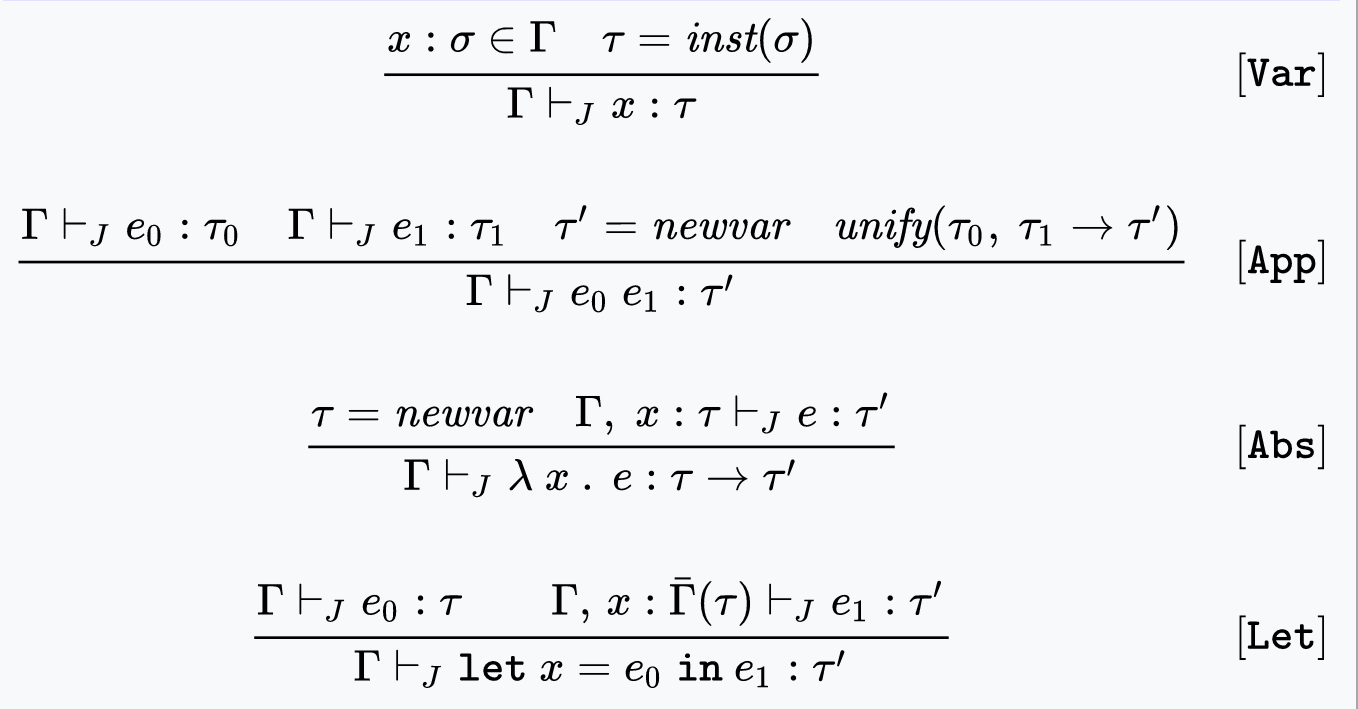
\includegraphics[width=0.9\linewidth]{hindley-milner.png}
  \end{center}
  \caption{A formal description of Hindley-Milner type inference, a core idea in ML family languages (from \citep{HindleyMilnerWikipedia})}
  \label{fig:hm}
\end{wrapfigure}


The tidal wave of interest in object-orientation in the early 1990s had significant impact in academia, just as in industry.  By the mid-1990s many in the world of FP and PL
were genuinely shocked, bewildered, disoriented and in some cases disillusioned by the rise of C++, Java and OO in general.  Reactions varied, and I now examine responses to
the OO tidal wave that are key to understanding the genesis of F\#, Scala and other languages in the 2000s. 

One response to object-orientation was to “give in” and work on Java implementations. Others worked on formalisms around Java, and indeed I initially
did just that for my PhD thesis \citep{Syme1999} and others formulated and published foundational object calculi. Some responded by integrating object-oriented
features into FP languages: LISP had already added CLOS, the Common LISP object system and OCaml saw the introduction of new forms of
genericity (“row-polymorphism” and “column polymorphism”) used as the basis for a fascinating object system \citep{Garrigue2001}. Around the same time the Standard ML
designers and implementers started an initiative called ML2000, whose aim was to use formal, theoretically-founded 
approaches to build a language to rival object-orientation. This effort foundered and stopped in the late 1990s.

Another response was to propose to integrate specific technical features associated with strongly-typed functional languages into “mainstream” OO
languages.  Wadler and Odersky led the charge with the development of Pizza, a variation of Java that incorporated parametric polymorphism (generics), discriminated
unions and first-class function values \citep{Bracha1998}.  This was subsequently trimmed-down to the proposal Generic
Java (GJ), and later heavily influenced C\#, Scala and F\#. Ultimately GJ became the basis for Java generics, though its use of “erasure” and lack of accurate
runtime type information were significant compromises. 

An alternative angle was to “deconstruct” functional programming itself and examine the underlying problems (as exhibited by implementations of Haskell
or Standard ML for example). One instance of this was the paper \textit{Why no one uses functional languages} \citep{Wadler1998}. This paper was central to
my understanding of the programming language landscape as I started at Microsoft Research in 1998.  Instead of blaming the unwashed masses for their
ignorance, Wadler’s paper outlines seven problems of strongly-typed FP implementations at the time: Libraries, Portability, Availability, Packagability, Tools,
Training, Popularity.  It also listed Performance and Ignorance as non-reasons. The early development of F\# was essentially an effort to address each of these.

Further, some responded by trying to compete via new commercial implementations of strongly typed FP languages including Poly ML and Harlequin MLWorks. However,
these saw little adoption and left the community with the feeling that the support of a “big player” in the industry was needed. 

A final response was to attempt to use the JVM as a substrate for implementing established functional programming languages, and thereby as a delivery
vehicle for FP into the browser and the web (the nascent driving force behind Java at the time).  Foremost in these efforts was MLj, a research/commercial
implementation of Standard ML by Benton, Kennedy et al. at Persimmon \citep{Benton1999}.  MLj was a whole-program compiler which allowed interop with the Java ecosystem through object programming extensions. When the research
arm of Persimmon folded in 1998, Benton moved to MSR Cambridge, followed later by Kennedy, bringing experience highly relevant to .NET and later F\#. Despite
these various responses, there was also strong anathema to object-orientation in theoretical communities: proponents of OO were too readily labelled with the
tar-brush of heresy: “unprincipled nonsense”, “lacking theoretical foundations” and similar.  

That completes our summary of the general surrounding context as I joined Microsoft Research in 1998 and began precursor work leading to F\#. For completeness,
the background influences I am aware of were as follows:

\begin{itemize}
\item I had used strongly typed functional programming, mostly in the context of theorem proving systems (Edinburgh ML in HOL88, Standard ML
of New Jersey in HOL90, Caml-Light in HOL-Lite, ForteFL at Intel). I had come to love them, while appreciating their weaknesses. In my undergraduate work
I had been supervised by one of the originators of ML, Malcolm Newey. Through my PhD work, the OCaml community and MSR Cambridge, I was
involved in overlapping communities that saw strongly typed functional programming as the norm.
\item I had used object-oriented languages (C++, Java) including studying Java and the JVM formally as part of my thesis work.  My
experience with C++ at university in 1992 had been negative, particularly through the over-use of hierarchical classification in student
projects---both as a modelling technique and its encoding in class hierarchies.  
\item As a child, from 1980-87, I had used BASIC and Logo (Apple II) and Turbo Pascal (Windows). As a student, I used Prolog, C, Scheme, Modula 2. A
comparative programming languages course provoked interest in a range of languages. In early employment I had used Prolog on Windows for an Australian
software company (SoftLaw, 1990-1993). 
\item I had implemented several strongly-typed language, proof and compilation systems as part of my PhD thesis work using various ML dialects and
toolchains including SMLNJ, MoscowML, Caml-light and OCaml. Additionally, I had, somewhat unusually for the times, also implemented some visual tooling
for these systems, notably a graphical proof editing IDE for HOL90 \citep{Syme1995} and a proof editing workbench for the theorem prover DECLARE \citep{Syme99threetactic}.  I
had a positive disposition to IDE tooling and understood the interaction between IDE tooling and language design.
\item In 1996-98, I had been exposed to the work of academic leaders such as Drossopoulou, Leroy, Wadler and Odersky to synthesize OO and functional
programming \citep{AlvesFoss1999}.
\item I was part of discussions trying to reimagine how we deliver strongly-typed functional programming to “the masses”.
\end{itemize}

\section{Project 7 and .NET Generics}

When Project 7 kicked off at Microsoft, the researchers at MSR Cambridge recommended the following languages for inclusion on the academic
stream: Eiffel, Mercury, Standard ML, OCaml, Scheme, Alice and Haskell.  The biases of the research group at MSR are clear here: 6 of 7 recommendations
were strongly typed languages, and 3 of 7 were firmly “strongly typed functional languages” in a specific sense of the term, e.g. incorporating Hindley-Milner
type inference and having functions as first-class values. Commercial languages in Project 7 included Perl, Python, Cobol and Ada. Academic or commercial
partners were found for each, funding was provided by Microsoft and workshops were arranged at MSR Cambridge and elsewhere.

In retrospect Project 7 was flawed but not catastrophically---some of the researchers didn’t engage, few of the language implementations saw much use, and
the costs to maintain them were high. While you can still buy and use Cobol.NET today, .NET programming is dominated by two Microsoft-supported
languages C\# and F\#, and the JVM has a more vibrant multi-language ecosystem. However Project 7 did have definite technical impact: for example, at
this stage, Gordon and Peyton Jones engaged with the designers of .NET, and argued successfully for the inclusion of tailcalls as a first class
operation (the “tail.” instruction in the .NET bytecode), both to support some of these languages and as a way of differentiating the .NET bytecode from the JVM.  This
started .NET down a long technical path of innovation and differentiation led by the demands of the languages being brought to the
platform.\footnote{Support for the “tail.” instruction remained patchy in .NET implementations for many years: convincing a team to ``innovate'' is one
thing, but delivering and maintaining the results requires ongoing commitment and costs.}

Project 7 also had an impact by raising the question of “language interoperability”: it was one thing to get languages targeting a common
substrate, another to get them to interoperate.  In 1999, I and colleagues wrote the internal whitepaper “Proposed Extensions
to COM+ VOS” \citep{GenericHistory} which argued that 

\begin{quote}
a primary objective of the COM+ Runtime is to deliver services and performance that are clearly technically superior to those provided by other potential backend runtime environments.\footnote{At this time, Project Lightning (i.e. .NET) was called “COM+”.  VOS is for Virtual Object System, the name of the .NET object system at the time.} 
\end{quote}
and that Microsoft should “get serious about language innovation”.  Five technical features were proposed, of which “generalized
delegates” (i.e. functions as first-class values) and “enhanced parametric polymorphism” were the more serious.  The influence of Pizza and GJ is strong here
and these are explicitly mentioned as competitors. I also developed ILX, an prototype extension to the .NET bytecode incorporating these features, which I hoped
might be adopted by other Project 7 languages. ILX was implemented on .NET by erasure and compilation to the existing .NET IL \citep{Syme2001}.


This whitepaper served as the start of the “.NET Generics” project, specifically designed to bring a form of generics to .NET that could work for both C\# and other
Project 7 languages such as Eiffel, OCaml and Haskell. .NET Generics and its history is covered elsewhere \citep{RefWarren} and over the next 4 years, Syme, Kennedy and Russo worked with
enormous dedication to deliver .NET Generics in C\# and .NET \citep{Kennedy2001}. The feature encountered enthusiasm, reluctance and indifference from
various parts of Microsoft, though a review to Gates in 2001 was well received and started to turn things around \citep{RefGatesReview}.   Anders Hejlsberg
was a key decision maker and my recollection is that much of the C\# language design work involved second-guessing how to shape the feature so it would meet approval. Ultimately the feature was
delivered as part of the 2005 .NET 2.0 “Whidbey” release.  At the same time, Microsoft began to make its first very tentative steps towards embracing open
source, and a “shared source” release of the .NET codebase was made called Rotor along with a corresponding extension containing the .NET Generics implementation
called Gyro.  A poster from MSR’s internal tradeshow “Tech Fest” is shown in Figure~\ref{fig:fig1}. 

\begin{figure}

  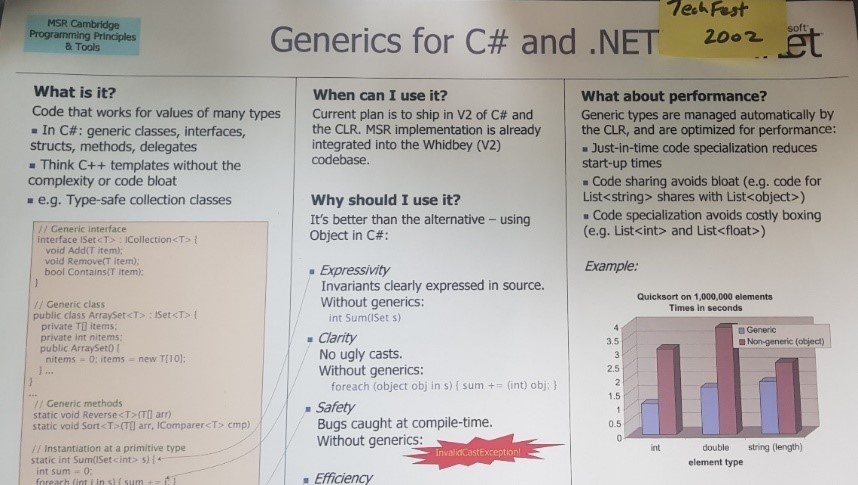
\includegraphics[width=0.8\linewidth]{fig1.jpg}
  \caption{.NET Generics poster at TechFest 2002, Microsoft Building 33, Redmond (photo by author)}
  \label{fig:fig1}
  \Description[.NET Generics poster at TechFest 2002, Microsoft Building 33, Redmond]{Shows information about .NET Generics - what it is, when it's useful and performance using a simple example.}
\end{figure}

The key premise of .NET Generics is that generic instantiations can be “managed” by the runtime environment, inclnuding the management of runtime type information
and the JIT-compilation of fresh code for newly encountered instantiations.  This avoids the need to either tag or box integers and other “unboxed” values---a technique
normally needed when combining polymorphism and separate compilation, because the runtime is able to specialize code on-demand.

This means the end-programming model in, say, C\#, can support a form of generics that is very complete and smooth from the programmer’s perspective:
runtime type information is accurate, the process of making and managing instantiations unobtrusive, the code for instantiations is automatically shared based on a
policy. .NET Generics has been successful: it is widely adopted by millions of C\# and F\# programmers; it is seen as a key differentiating factor of C\# over Java; and
has been the basis for many later innovations delivered in F\#, C\# and .NET. For example, generic collections (C\# 2.0), LINQ (C\# 3.0), tasks (C\# 4.0),
async/await (C\# 5.0) and Span (C\# 7.2) all use .NET Generics heavily, as do all F\# features. .NET Generics put .NET years ahead and even today systems such as
Java and Go struggle with the implementation of aspects of genericity such as supporting instantiation at both reference and value
types \citep{RefValhalla, RefGoGenerics}.\footnote{In \citet{RefGoGenerics2} the designer of Go, Rob Pike, is quoted \textit{The time has come to change Go, given what we have learned
over the past decade of using it in production. It’s going to take a long time to sort this out. It could be
years before anything is really resolved so...Please be patient.}}
Equally, generics is a technical feature that imposed significant costs on Microsoft’s .NET implementation going forward. Generics is most easily implemented via a JIT and attempts to do fully
static compilation of .NET code have struggled with the feature.


From the perspective of the history of F\# (which did not yet exist), the successful delivery of .NET Generics intentionally made .NET a suitable substrate
for a “direct” compilation from a strongly typed functional language into .NET bytecode: this was by design, not by accident. For example, it allowed a simple, direct
compilation of genericity inferred via Hindley-Milner type inference into .NET Generics with little or no runtime overhead.  Consider simple code such as this in some ML-like dialect:
\begin{verbatim}
    let keyAndData getKey x = (getKey x, x)
    let data = [| 1 .. 100 |]
    let add x = x + 1
    let y = Array.map (keyAndData add) data
\end{verbatim}

Here the generic code has been instantiated at integer type. In many systems of generics such as GJ, values of generic type such as
parameter \texttt{x} to \texttt{keyAndData} would be represented in boxed (heap-allocated) form.  Thus, in the absence of other optimizations, the code
above would cause the boxing of the integers as they enter the (generic) \texttt{keyAndData} function, and then unboxing as they are passed on
to the (non-generic) \texttt{add} function.  Such implicit costs for basic collection types would be unbearable and make any Hindley-Milner type-inferred language
intrinsically low-performance on .NET. With .NET Generics these specific performance problems go away.  In crucial ways .NET Generics laid a foundation for later work on F\#.


\section{The Decision to Create F\#}

At MSR, Project 7 also led to the SML.NET project \citep{Benton2004}.  SML.NET was a continuation of MLj, mentioned earlier, retargeted to
.NET.  SML.NET used a sophisticated whole-program optimizer and was a faithful implementation of Standard ML
with extensions for object programming. The system was of high quality but didn’t gain significant external mindshare.   During 2001, I grew frustrated with SML.NET,
which was not yet released even though .NET itself was now public. While respecting the research goals of my colleagues, I was keen to see strongly typed FP delivered
in a way that could be readily adopted by large numbers of programmers, and on a path to addressing the seven major themes identified by Wadler in 1998 \citep{Wadler1998}.  The
implementation of OCaml was influential on me here: OCaml used a relatively direct and simple compilation strategy, and it was not clear that a whole-program
compilation strategy was needed to achieve acceptable and reliable performance.  Further, SML.NET didn’t target .NET Generics, and there was no definite plan to
make it do so: the compiler was predicated on the benefits of whole-program compilation and pervasive monomorphization, with the aim of recovering performance
and compact code.  As commonly happens in research labs, a divergence of opinion occurred.


Initially, in late 2000, in conjunction with Reuben Thomas, I attempted an implementation of Haskell for .NET, using a direct translation from the “Core” intermediate
representation of the Glasgow Haskell Compiler (GHC) to the .NET bytecode. This experience was partly successful: small programs ran. However, the advice of Simon
Peyton Jones led me to believe that Haskell.NET couldn’t be successful for several technical and cultural reasons:\footnote{See also the later
summary \textit{Why isn't GHC available for .NET or on the JVM?} \citep{RefGHCDotNet}.}

\begin{itemize}
\item As with other Project 7 languages, running Haskell on .NET “in isolation” was not enough in itself: a primary goal was to make a functional language that
was fully part of the .NET ecosystem, with full interop with .NET libraries. 
\item Full interop means that every .NET function would need a rendering in Haskell with a Haskell type, so type translation is needed. The type systems
were not the same, so the translation is onerous or simply impossible in many cases.  
\item Moreover, to ease the translation, Haskell itself would need to be adapted to incorporate some form of subtyping and object programming and would
eventually need the ability to extend an existing .NET class.   The Haskell community was reluctant to contemplate such substantial language changes driven
by the requirements of a particular platform. 
\item At the time, almost all Haskell code (if you include libraries) needed technical features that lacked corresponding .NET support, including higher-kinded
type variables, lightweight concurrency, exceptions (with Haskell’s exception semantics), ephemerons and software transactional memory. So, even interop
aside, it would be hard to claim that any Haskell program would run well on .NET; only a subset would do so.   
\end{itemize}
So, work on Haskell.NET stopped in late 2000.

The question of OCaml and JVM/.NET was also being discussed on the Caml mailing list around this time.  An example is the following message from
myself, on February 6, 2001 \citep{RefCamlArchive1}:
\begin{verbquote}
Subject: OCaml on CLR/JVM? (Was RE: OCaml <--> ODBC/SQL Server)

> What I cannot find around is a way to easily interrogate and interface 
> in OCaml with an ODBC data source...

Now I have to say the obvious: wouldn't it be wonderful if Caml interfaced with either Java or the .NET Common Language Runtime seamlessly so we wouldn't have to keep facing these kinds of questions and problems, and could just leverage existing libraries?   

I'm very interested to know if there are people with some time to spare who would be keen to work with me toward a .NET version of OCaml.  I've talked this over from time to time with Xavier, and have done a lot of foundational work for the core language when building a .NET compiler for Haskell.  If you think would be interested, or would simply like to join a mailing list devoted to talking about getting Caml running and interoperating on .NET, then please let me know!
\end{verbquote}
This was the first explicit public indication of my desire to create a version of OCaml targeting .NET. Leroy replied on February 8, 2001 \citep{RefCamlArchive2}:
\begin{verbquote}
I've been working on and off (mostly off, lately) on an OCaml/Java interface that works by coupling the two systems at the C level via their foreign-function interfaces (Java's JNI and OCaml's C interface).  This was strongly inspired by the work of Erik Meijer et al. on a similar Haskell/Java interface.  (These Haskell guys sure are at the bleeding edge of language interoperability.  This is the second interop idea I steal from them, after the IDL/COM binding.)

The low-level coupling is surprisingly easy, including making the two garbage collectors cooperate: both the JNI and OCaml's C interface provide enough functionality to get the coupling to work without *any* modification on either of the implementations.  How nice! The only limitation is that a cross-heap cycle (a Java object pointing to a Caml block pointing back to the Java object) can never be reclaimed... (Thanks to Martin Odersky for pointing this out.)

Of course, the low-level interface is type-unsafe, so the real fun is to build a type-safe view of Java classes and objects as Caml classes and objects, and conversely.  I'm still struggling with some of the issues involved.  For instance, it turns out to be much simpler (for the implementation, not for the final user!) to map Java objects to values of abstract Caml types, and treat methods as functions over these abstract types, than mapping Java objects to Caml objects.  That was quite unexpected!

One thing I learnt is that the real problem with language interoperability is not how to compile language X to virtual machine Y (this can always be done, albeit more or less efficiently), but rather how to map between X's data structures and objects and those of all other languages Z1 ... Zn that also compile down to Y.  This is obvious in retrospect, but I think many (myself included) often overlook this point and believe that compiling to the same virtual machine is necessary and sufficient for interoperability.  It is actually neither necessary nor sufficient...

While this work started with the JVM, I'm pretty sure it can be made to work with the .NET CLR, as soon as it will have a foreign-function interface with features comparable to those of the JNI.  (And I'm sure this will happen eventually, not only because it makes sense, but also because Java has it, so .NET must too :-)

Stay tuned for further developments.
\end{verbquote}

This lays out the basic question many languages have faced since: should a language have its own runtime and interoperate indirectly with .NET and/or the JVM, or
should it target those runtimes directly?\footnote{Interestingly, this discussion arose directly in the context of data integration, an area that would drive much
of the C\# and F\# design work in the 2000s.}  Leroy’s response represented a divergence of opinion: Project 7 had envisaged very close interoperability, sharing
one virtual machine including memory, code, reflection, JIT, GC and library capabilities, and potentially bringing the object system of the host ecosystem into the
language.  The approach described by Leroy was, technically, highly sensible for the existing OCaml implementation, however it didn’t feel right once .NET could be
assumed. To me, it would intrinsically run into performance, interoperability, tooling and other issues at boundaries between the languages, and adoption would be
limited to the intersection of those willing to rely on both the .NET and OCaml implementations.

The discussion also brought contributions from Dave Berry, based on his prior experience of implementing
Harlequin’s MLWorks \citep{RefHarlequin}, a proprietary
implementation of Standard ML (Dave later contracted with MSR Cambridge on an open source version of .NET Generics), on February
9, 2001 \citep{RefCamlArchive3}:
\begin{verbquote}
> > Now I have to say the obvious: wouldn't it be wonderful if Caml interfaced with either 
> > Java or the .NET Common Language Runtime seamlessly so we wouldn't have to 
> > keep facing these kinds of questions and problems, and could just leverage existing 
> > libraries?   

Although this view is understandable, I think it is rather naive. ... To look at it another way, OCaml already shares a platform with C (at least with the native-code compiler), so all the C libraries are already available... Yet it can still be a lot of effort to link with a C library.  Why should Java and .NET be any easier?  Also, look at the effort that went into making an ML/Java system with MLj... Threads are another area of potential problems.  In fact they can be a total minefield.
\end{verbquote}
To which I replied on February 10, 2001 \citep{RefCamlArchive4}:
\begin{verbquote}
There's hard work to be done to realise this vision, but in principle a clean interop story sure beats the endless rehashing of other people's code in language X as a library in language Y.  Myself and others involved in the Project 7 are working on one approach to achieve this interop, i.e. compiling languages directly to .NET MS-IL, in the style of MLj, often adding extensions to the language in order to improve the interop.  We are also working on improving the .NET infrastructure, proposing support for features such as parametric polymorphism in MS-IL.  

Xavier is also working on a solution for OCaml, as he mentioned, though the problem of how to reflect the constructs of an object model into ML, Haskell or OCaml remains similar whichever approach you take to actually running the stuff.

There are several reasons why it is easier: exceptions, for example, can be propagated across the interop boundary, without any effort at all if you compile to MS-IL or Java bytecode.  If you're compiling to bytecode you can also ensure more compatibilities of representations, e.g. make sure ML int64's are exactly representationally equivalent to C's int64s.  Note if you don't compile to a bytecode then you even have to marshal integers across the interop boundary in Caml, though this could be automated.

You can also transfer objects more consistently, as the semantics of the object models of Java and .NET are fairly simple in contrast to C, e.g. no need to have an IDL to help interpret pointers as "in-out", "in", "out" parameters.

While at a certain level I like Xavier's approach, i.e. maintaining two runtimes, garbage collectors etc., I have troubles seeing it scaling to the multi-language component programming envisioned as part of .NET approach (and indeed currently in practice with C\#, C++, VB.NET and other .NET languages).  Two GC's are already trouble enough (performance might suck as they will both be tuned to fill up the cache), but if you have components from 10 languages in one process?  10 GCs competing for attention?  Maybe it can be made to work, but there's a certain conceptual clarity in just accepting that a GC should form part of the computing infrastructure, and share that service.  These are the aspects of the .NET approach that I find quite compelling.

As an aside, I think it would be an interesting question to say "OK, let's take it for granted that the end purpose of our language is to produce components whose interface is expressed in terms of the Java or .NET type systems, but which retains as many of the features and conceptual simplicity of OCaml and ML as possible."  I'm not sure exactly what you'd end up with, but whatever it was it could be the language to take over from C\# and/or Java (if that's what you're interested in...)  But without really taking Java/.NET component building seriously right from the start I feel you're always just going to end up with a bit of a hack - an interesting, usable hack perhaps, but not a really good language.

Probably the greatest recurring technical problem that I see in this kind of work is that of type inference, and the way both the Java and .NET models rely on both subtyping and overloading to help make APIs palatable.  Type inference just doesn't work well with either subtyping or overloading.  This is a great, great shame, as it's obviously one of the main things ML has to offer to improve productivity.  

P.S. As for threads - I don't think the story is half as bad as you might think.  After all, OCaml threads map down to Windows threads at some point, and I just don't see that there are that many special logical properties of typical ML and Caml threading libraries that make it semantically ridiculous to share threads between languages (though it is true asynchronous exceptions can make things hard when compiling to a bytecode).  But I'll admit I'm not an expert on this. 
\end{verbquote}
Finally, there was techno-political controversy too, this time in a reply from Fabrice le Fessant on February 12, 2001 \citep{RefCamlArchive5}:
\begin{verbquote}
Is the .NET VM open source ? Which part is Microsoft-independent ?...

If Microsoft wants its new product to be used, it is Microsoft problem to port more languages to its VM, and not only say: "We have ported our homemade languages to it (C\#, C++, VB.NET) [because it was designed for them], so, you see, we have proved it's the universal VM. Now, do the same for your languages, or your language will not be used anymore by our customers..."

So, why do we really need a .NET port of OCaml ? OCaml is working fine on Windows, and on many other OS ... 
\end{verbquote}
A discussion thread followed on the merits of open source, standards, interoperability and cross-platform execution, issues which weren’t resolved for F\# for another 13 years, when F\#, C\# and .NET Core were finally open source and cross-platform.  A contribution by Dave Berry on February 16, 2001 was more positive \citep{RefCamlArchive6}:
\begin{verbquote}
I think Microsoft should be congratulated on their outreach to programming language researchers.  I for one would certainly welcome a widely distributed VM that is a good target for compiling ML.  Interoperability with other languages on the same VM would be a bonus... That said, interoperability is still hard...
\end{verbquote}
There were many valid arguments and sensitivities here, and I proceeded from this point determined to be highly respectful towards OCaml and its existing user base: I genuinely loved the language and the approach to programming it represented. 

Predicting the future trajectory of software infrastructure like .NET and architecture was also an important factor in making decisions, e.g. in this final response by Arturo Borquez on March 3, 2001 \citep{RefCamlArchive7}:
\begin{verbquote}
Perhaps I am wrong, but let me state what I believe about this stuff.... C\# is not really important as it will never reach the 'mass' of VB... The real issue is ... the Client/Server model ... In my opinion this model has no future, ...clients would become minimal.... with a diverse and broad family of client devices (terminals). My conclusion is CLR/JVM ... are not important for the future of Caml, as all will die. Caml will need only some library updates to match the communication tech upgrades.  
\end{verbquote}
In hindsight, predictions like these were both right and wrong: the structure of applications evolved extensively, and .NET and the JVM ultimately de-emphasized their role as “middleware”, but neither .NET nor the JVM have died.  Languages and runtimes seem to endure longer than software architectures.

In mid-2001 the itch remained: how was MSR going to bring strongly typed functional programming to .NET in a way that could be readily adopted by large numbers of programmers?  By October 10, 2001 I felt firm enough in this conviction to reply as follows:

\begin{verbquote}
When time permits I plan to implement a .NET CLR compiler for Caml. Initially I will implement only the core language, and perhaps first-order modules, and then to assess things after that.  I will be coding the implementation up from scratch rather than using the sources for the existing OCaml compiler...

My first reason for doing this is because I have an existing OCaml code base that I would like to make available as a .NET library...  Plus I love Caml, and would like to see it supported on .NET, and I'm interested in proving that interoperability between functional languages is practical in .NET. 

This implementation path would give object introspection capabilities for free.  However it would no doubt be slower than the existing native code Caml implementation: you don't get something for nothing.

I don't know of any other active efforts to do a .NET compiler for Caml.  SML.NET will, hopefully, be available publicly soon.
\end{verbquote}
So, by late 2001, a viable path appeared possible: to bring a variant of the OCaml language to target .NET itself. The Project 7 effort around OCaml
had led to the above approach by Leroy and didn’t look likely to continue.  This left a space for a new Caml.NET initiative, though one targeting
the .NET IL itself, and in December 2001 I decided to move ahead with an “Caml.NET”. This was later rebranded “F\#” after private discussion with
Cedric Fournet and Georges Gonthier, to allow for greater divergence from OCaml and to bring language experimentation into
scope.\footnote{The “F” in “F\#” comes from both “Functional” and “System F”, an elegant variant of simply typed lambda calculus. Today an F\# community saying “F is for Fun”.}


\section{Early F\#---2002--2003}

The early conception of F\# was simple: to bring the benefits of OCaml to .NET and .NET to OCaml: a marriage between strongly typed functional
programming and .NET.  Here “OCaml” meant both the core of the language itself, and the pragmatic approach to strongly-typed functional programming
it represented. The initial task was relatively well-defined: I would re-implement the core of the OCaml language and a portion of its base
library to target the .NET Common Language Runtime. The implementation would be fresh, i.e. not using any of the OCaml codebase, for legal clarity. 

The first lines of the F\# implementation were written in December 2001, a front-end for a re-implementation of the core Caml syntax targeting ILX as a back end, and thus to .NET. The initial compiler was written using OCaml (later bootstrapped using F\# in 2006). 

The initial design choices were subtle.  By far the most wide-ranging design decision is easy to miss in retrospect: after choosing OCaml as a
starting point, the most significant design choice made for F\# was that it be a .NET language.  Everything else was to be subservient to
that goal.  In particular, .NET types are F\# types, .NET values are F\# values, .NET exceptions (and their semantics) are F\# exceptions
(and their semantics), and .NET threads are F\# threads.  The same was true in reverse and “two-way interop” was always a design goal.
There’s no type translation, no marshalling from one representation to another. Strings in F\# were to be strings in .NET and vice-versa.
Types and functions defined in F\# could be used from other .NET languages. This decision gave F\# less room to innovate---more often
than not, F\# is stuck with whatever .NET does---but it guaranteed two-way interop.  This was a huge reason for starting a new language
design, rather than trying to map an existing language onto .NET.  This full identification of types and data goes beyond the question of
having one runtime vs two: even if you have one runtime, a language could still have chosen to use different representations for (say) a
list of integers, represented internally as .NET objects of some kind, but marshalled when passed to a .NET method: one runtime, but two
representations. F\# doesn’t do that: it uses one runtime and, where possible, identical representations. This influenced many small decisions: for
example, from the outset a function declared in F\# had a guaranteed, stable representation in .NET code as a static member of a class with a
stable name, and could be used directly from .NET languages.  This also meant F\# code could always be accessed via .NET reflection.  Although
the first version of F\# was initially presented as “Caml-for-.NET”, in reality it was always a new language, designed for .NET from day 1. F\# was never
fully compatible with any version of OCaml, though it shared a compatible subset, and it took Caml-Light and OCaml as its principal sources of design guidance and inspiration.  

%\begin{wrapfigure}{R}{0.5\textwidth}
 % \begin{center}
 % 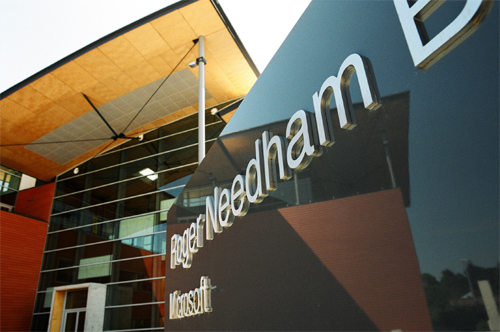
\includegraphics[width=0.9\linewidth]{msft.jpg}
 % \end{center}
 % \caption{Microsoft Research, Roger Needham Building, Cambridge, UK, circa 2003 (credit: }
 % \label{fig:msft}
%\end{wrapfigure}


In addition, there was the question what not to implement.  A notable omission from the design was the functorial module system of
OCaml.  Functors were a key part of Standard ML and a modified form of the feature was included with OCaml, a source of ongoing
controversy amongst theoreticians.  I was positively disposed towards functors as a “gold standard” in what parameterization could
be in a programming language, but was wary of their theoretical complexities. Furthermore, at the time there were relatively few places
where functors were used by practicing OCaml programmers. One part of the OCaml module system---nested module definitions---was
eventually included in the design of F\#.  However, functors were perceived to be awkward to implement in a direct way on .NET and it
was hard to justify their inclusion in a language design alongside .NET object programming. Another decision was not to include any
OCaml 3.0 features, specifically neither the object system nor the recently added “named arguments” feature.  Leroy’s email above explains
the issues regarding the object system: there was sufficient disparity and mismatch between the object systems of .NET and OCaml that
the latter couldn’t be used for the former.  The OCaml pre-processor CamlP4 was also not supported, though CamlLex and CamlYacc could
be used. The question of the object system would be dealt with later.  However, this meant that F\# and OCaml diverged as of the core language of OCaml 2.0.


The first release (v0.1, soon replaced by 0.5) was made near-silently on June 4 2002 as an addition to the ILX project, making the following
claims on the website \citep{RefIlxPage}:
\begin{verbquote}
Mixed functional/imperative programming is a fantastic paradigm for many programming tasks....You can access hundreds of .NET libraries using F#...F# is an implementation of the core of the Caml programming language for the .NET Framework, along with cross-language extensions. ...The aim is to have it work together seamlessly with C#, Visual Basic, SML.NET and other .NET programming languages...Types and values in an ML program can be accessed from some significant languages (e.g. C#) in a predictable and friendly way. ...F# provides an implementation of a subset of the OCaml libraries as well as the ability to access .NET libraries.  Using the .NET libraries is optional.... F# supports features that are often missing from ML implementations such as Unicode strings and dynamic linking... Tooling consists of a simple command line compiler, supporting separate compilation, debug information and optimization... F# is, as far as I know, the first ML compiler to have good binary-compatibility and versioning properties....
\end{verbquote}

Some hurdles had been cleared along the way. MSR granted permission to allow commercial use of programs compiled with ILX and this
permission was recycled for the F\# implementation. Next, at a conference I asked Leroy for tacit approval in putting out a variant of
Caml for .NET, including making changes to the language design.  Leroy approved---OCaml itself was part of a long history of adapting
and modifying the core ML---and what was research if we didn’t experiment?  In a later email reply Leroy said:

\begin{verbquote}
Don Syme and his Microsoft Cambridge colleagues did a great job with adding parametric polymorphism to the .NET framework -- something that was initially overlooked in .NET --, and I'm very happy that they chose core Caml to demonstrate this extension in action. https://caml.inria.fr/pub/ml-archives/caml-list/2002/06/8d07fd5058aa26127d1b7e7892698386.en.html 
\end{verbquote}
To which I replied \citep{RefCamlArchive8}
\begin{verbquote}
And I'm even more grateful to Xavier and the team for doing such a great job with OCaml over the years, and for providing a solid core language, an excellent runtime system and the very interesting set of language features they've added to the core.  Core Caml provides a great starting point for work of all kinds: I used it in my PhD thesis, for example, as the term language for a theorem prover.

I chose to implement a core Caml compiler for .NET partly to test out generics, but also because I want to be able to program against .NET libraries using the language I love to program in, and reuse the libraries and techniques I've developed.  I guess it's possible I'll get a bit of flak from the Caml community about F#.  Being at Microsoft Research I presume I'll be writing a fair bit of .NET code sooner or late, and personally I'd rather do that in Caml/F# than C#... I hope the Caml community won't mind me making that opportunity available to others via the public release of F#.  
\end{verbquote}
The first real design-work began with the addition of the ability to access .NET object types via the dot-notation.:
\begin{verbquote}
C# and other .NET languages can be directly accessed from F#...  Types are accessed using the "Namespace.Type" notation.  You may simply use "Type" if an "open Namespace" declaration has been given. Instance members are accessed using "obj.Method(arg1,...,argN)" or "obj.Property" or "obj.Field". Static members are accessed using "Namespace.Type.Method(arg1,...,argN)" or "Type.Method(arg1,...,argN)", similarly for properties and fields. 
\end{verbquote}

While seemingly innocuous, this design decision broke with OCaml and a long tradition of ML language design: it used inferred type information in name resolution. A name like M in obj.M was now resolved immediately using the partially inferred type of obj rather than by adding a new inference constraint. This meant that type annotations would now sometimes be needed, compromising one of the traditional “rules” of ML (i.e. that type annotations are strictly optional), and that inference becomes “algorithmic” or “left-to-right”:

\begin{verbquote}
Typing. Sometimes extra annotations are needed to get the program to typecheck, e.g. casts using "(cast <expr> : <type>)" and type annotations to help resolve overloading.
\end{verbquote}

I decided that if the inference algorithm was well-defined and kept stable, this would be sufficient for interoperability purposes. In
practice, the use of partially inferred type information in name resolution proved effective and stable and was kept throughout the
evolution of F\#.  Type inference was eventually specified algorithmically in the language specification. 

Another design question was about nulls. The question was not one of safety: like the JVM, the .NET runtime would itself perform null
checks when values were accessed. Instead, it was a matter of program correctness. The SML.NET system had “sanitized” all interop
calls by inserting the Standard ML “option” type with tags SOME/NONE at all relevant points.  In F\#, I decided not to do this:
\begin{verbquote}
Null.  Null objects returned by the .NET assemblies are NOT checked by the process of importing the assemblies or by the F# type system.  This may be addressed in the future, but for the moment use the "nonnull" function from Pervasives to check if values are null and the "null" value from Obj to create a new null value. https://web.archive.org/web/20020814185220/http://research.microsoft.com:80/projects/ilx/fsharp-manual-import-interop.htm
\end{verbquote}
Instead, the rule adopted was that .NET-declared types would allow the use of “null”, while F\#-declared nominal types would not.  This
kept a strict approach to nullness within F\#-only code, in keeping with OCaml but allowed the use of null in interop scenarios with .NET
types. This was partly because of ergonomics: the insertion of the option type was highly intrusive on programming and nulls were not
used as pervasively in the .NET libraries as in Java, so in balance the need for a pleasant programming experience outweighed the need
for null-safety at interoperability. Further, I felt that the topic of null-safety should be dealt with systematically across all .NET languages, as
we had done with .NET Generics.\footnote{This position eventually bore fruit in 2018 when C\# 9.0 finally began the transition to assuming
non-nullness by default for reference types, discussed in the retrospective.}   

Initially, early F\# avoided adding object programming declarations:
\begin{verbquote}
Currently you cannot declare new classes or implement interfaces in F#.  For the moment workaround this by declaring a new class in C# that accepts delegate parameters to implement the virtual/interface members, and then pass function values from F# to the C# class.  You will only need to write this C# class once.
\end{verbquote}

Further, contrary to the warnings from Dave Berry and others in the email threads shown earlier, no design work was needed for threading: F\# simply assumed the same threading model as .NET itself, which essentially mapped .NET threads to operating system threads.



\section{Early F\#---Release}


F\# “0.5” was little noticed at first, deliberately: the initial implementation was lacking in many ways and needed time to settle. Initially, the plan was as follows: 
\begin{enumerate}
\item Make the language viable for adoption and use.
\item Use it to stress-test .NET Generics.
\item Get it out to the public.
\item See where things led.
\end{enumerate}

I had been influenced by my time at Intel Strategic CAD Laboratories, which used a structured “maturity model” for research projects and
technology development: projects at Intel would proceed from “concept” to “proof of concept” to “prototype” and then through a product
delivery phase. Thus there was no Microsoft “buy-in” at this stage: few at the company knew of F\# apart from those in MSR Cambridge
and their .NET team contacts. 6 months later, after several iterations, the project got noticed by Internet news sites, always keen for the
latest scoop, and I decided to make a clarification on the OCaml mailing list in case things “got out of hand” before the implementation was fully
ready, and in case accusations of “embrace, extend, extinguish” emerged \citep{Boulton2003}.

\begin{verbquote}
There have been some utterly speculative (and entirely off-the-mark!!) internet press reports about this project in the last few days (e.g. see internetnews.com).... I thought it wise to add the following clarification to the F# website and to post it to this list.

...Despite reports suggesting otherwise, F# is a relatively small research project designed to demonstrate that it is possible to easily implement ML-like languages for use on the .NET Framework.  There are no current plans to commercialize F#.... F# is public, on-going research, and Microsoft Research regularly and openly collaborates with universities on programming languages
\end{verbquote}

The fact that F\# needed to be down-played initially was partly due to the sensitivities around launching anything “product-like” at the
time from MSR.\footnote{One reviewer queried whether the final statement about ``no current plans to commercialize'' was accurate
when written.  I can confirm this was the case: there was no plan at the time to commercialize F\#, either as part of Visual Studio nor any
other path. There were a vague aspirations on the part of the author (and the MSR managers who approved the release) that it might
prove commercially relevant.} At the time, all public software by MSR had an awkward legal/commercial status: publication of software
was primarily to support a research/publication agenda. Despite a budget nearing \$1B, the organization was not at that stage permitted
to make and release commercial products.  MSR strongly encouraged open research, but open software was more problematic. However,
designing and delivering new programming languages was an essential part of any PL research agenda, and indeed the whole rationale
behind Project 7.  Further, external “proofing” of these technologies was critical to refine them. 

External perceptions were also tricky to manage: from the perspective of computer science academia and hacker culture, corporations
in general---and Microsoft in particular---were often seen as structural adversaries. Offerings from MSR were even feared, and one
leading researcher suggested that F\# would “kill off” language research.  In retrospect such ideas seem laughable---PL research has
bloomed in the last 15 years and hundreds of new languages have been developed---but these views stemmed from anti-commercial
biases, fear of a perceived monopolist, and Microsoft’s opposition to open source software at the time. 

Either way, my belief was that, in the area of programming languages, you had to go public and be commercially usable in order to influence
programming practice, and to be true to both the spirit of research and the original goals of Project 7. Later, other cutting-edge MSR
projects would not reach their full potential, because they didn’t make the commercially usable releases necessary to proof the technologies
and gain evidence of their utility in sufficient time to occupy a market niche, examples include Accelerator and Dryad LINQ. On the other
hand, MSR provided a good “institutional home” for a language, given its concentration of expertise and its long-term mission to change
computing. Lab directors and managers such as Andrew Herbert, Andrew Blake, Luca Cardelli and Byron Cook would be consistently supportive of the work
on F\# over a long period of time. However, doing a public, commercially usable language offering via MSR was not going to be plain
sailing, and the support of the product teams would ultimately be needed.

\section{F\# 1.0, 2004--2006---Overview}

After completing .NET Generics in mid-2004, the rest of the year saw intense work on improving F\#. At this stage, .NET was on the
ascendency inside Microsoft and it achieved widespread external success on the back of a huge evangelization effort: most programming
for the Windows platform moved over to C\# and .NET worldwide. A massive shift towards .NET also happened internally: the Windows
team started major initiatives, including a rewrite of the Windows “shell” and the creation of many major .NET projects such as Windows
Presentation Foundation, Windows Communication Foundation and Windows Workflow Foundation.

On January 5, 2005, a pre-release of F\# 1.0 was declared in my first MSDN (Microsoft Developer Network) blog
entry \citep{RefBlog1}.\footnote{At the time, individual blogging on MSDN was encouraged by management and proved a positive way for those involved with F\# to utilize Microsoft’s positive brand with developers.}
In March 2005, F\# 1.0 was first demonstrated at “TechFest”, an internal MSR trade-show in Redmond.  

\begin{figure}
  \centering
  \begin{subfigure}[b]{0.47\linewidth}
    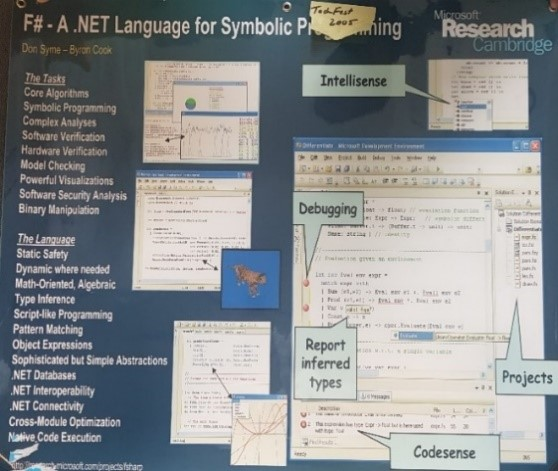
\includegraphics[width=\linewidth]{fig2a.jpg}
   \Description{A poster showing information about F\# including its relationship to other languages, its safety properties.}
  \end{subfigure}
  \begin{subfigure}[b]{0.47\linewidth}
    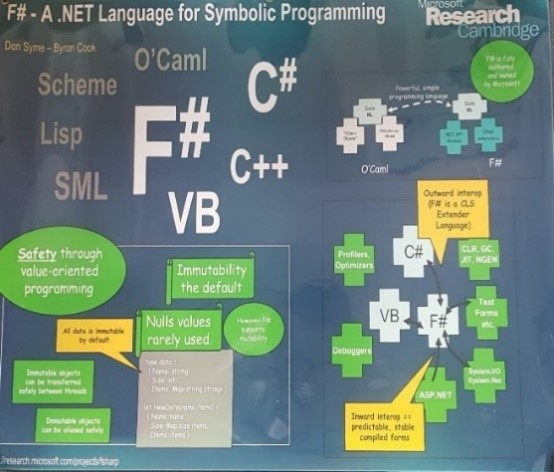
\includegraphics[width=\linewidth]{fig2b.jpg}
   \Description{A poster showing information about F\# including its relationship to other languages, its safety properties.}
  \end{subfigure}
  \caption{Two posters for F\# 1.0 at MSR TechFest 2005  (photos by author)}
  \label{fig:fig2}

\end{figure}


F\# developed in crucial ways during 2004-06.  Based on successful trials, and with the support of Byron Cook, MSR manager Luca Cardelli
agreed to add developer support to the project. On February 10, 2005 we were able to advertise and on 24 March 2005, James Margetson
joined to form a small team with interns (Dominic Cooney, May-July 2004, Gregory Neverov June-August 2006). Small internal and external
user communities grew and trust in the project began to form. The technical additions made to F\# during this time were as follows:

\begin{enumerate}
\item Completion of the core Caml-like language programming model (2004)
\item Targeting .NET generics (2004)
\item Addition of initialization graphs (2004)
\item Addition of method overload resolution and object-expressions for interoperability with .NET (2004)
\item Addition of “statically resolved type parameters” for handling overloaded arithmetic in a way that fits with Hindley-Milner type inference (2005)
\item Addition of class/interface constructs for object programming (2005)
\item Addition of implicit class construction (2006)
\item Addition of the “light” indentation-aware syntax (2006)
\item Addition of a treatment of subtyping within Hindley-Milner type inference (2006)
\item Addition of runtime meta-programming via quotations (2006)
\item Addition of F\# Interactive, a REPL for F\# (2006)
\item Initial Visual Studio tooling (2006)
\item Bootstrapping (2006)
\item Execution on Linux using Mono (2006)
\end{enumerate}

\begin{wrapfigure}{R}{0.5\textwidth}
  \begin{center}
  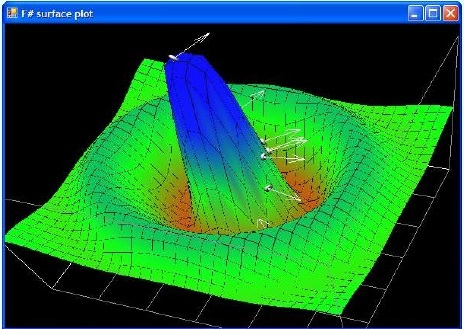
\includegraphics[width=0.9\linewidth]{directx2.jpg}
  \end{center}
  \caption{The ``DirectX 3D'' demo used in early F\# evangelism (screenshot by author)}
  \label{fig:directx}
  \Description[Screenshot of DirectX demo]{Screenshot of DirectX demo used in 2007}
\end{wrapfigure}

To “proof” the language we turned to some existing OCaml codebases at MSR including the SPiM (Stochastic Pi Machine), Static Driver Verifier
and Terminator projects.  These tests were successful, for example allowing the addition of a Windows-based GUI to SPiM.   During this time,
James Margetson was responsible for performance testing and supporting the internal use of F\# on these projects by Andrew Phillips, Jakob
Lichtenberg and Byron Cook. Margetson also implemented the first REPL for F\# and created numerous compelling demonstrations of interactive
development using F\# scripting and the REPL, including the famous ``DirectX'' scripting showing playful interactive construction of a 3D graphics scene, see
Figure~\ref{fig:directx}.
The author and Margetson were responsible for documentation and releases. Andrew Herbert and Luca Cardelli were the responsible MSR managers at this time.

During this time F\# was not the result of a “meeting of minds” amongst MSR Cambridge language researchers, but rather myself and collaborators
pursuing a series of design additions to the initial implementation, with the help of some feedback from colleagues, users, researcher networks
such as WG2.8 and an emerging worldwide community.  The design conversations in the external community on mailing lists and in blog responses
were encouraging, and internal and external adoption was growing steadily. 

\subsection{F\# 1.0---Pipelines}

One of the first things to become associated with F\# was also one of the simplest: the “pipe-forward” operator, added to the F\# standard library in 2003:
\begin{verbatim}
    let (|>) x f = f x
\end{verbatim}
In conjunction with curried function application this allows an intermediate result to be passed through a chain of functions, e.g.
\begin{verbatim}
    [ 1 .. 10 ] 
        |> List.map (fun x -> x *x) 
        |> List.filter (fun x -> x % 2 = 0)
\end{verbatim}
instead of 
\begin{verbatim}
    List.filter (fun x -> x % 2 = 0) 
       (List.map (fun x -> x *x) [ 1 .. 10 ])
\end{verbatim}
Despite being heavily associated with F\#, the use of the pipeline symbol in ML dialects actually originates from Tobias Nipkow, in
May 1994 (with obvious semiotic inspiration from UNIX pipes) \citep{RefPipeline, RefIsabellInfix}.
\begin{verbquote}
... I promised to dig into my old mail folders to uncover the true story behind |> in Isabelle/ML, which also turned out popular in F#...

In the attachment you find the original mail thread of the three of us [ Larry Paulson; Tobias Nipkow; Marius Wenzel], coming up with this now indispensable piece of ML art in April/May 1994. The mail exchange starts as a response of Larry to my changes.  

...Tobias ...came up with the actual name |> in the end...
\end{verbquote}
The use of the pipeline symbol is particularly important in F\# because type-inference is propagated left-to-right and name resolution occurs based on information available earlier in the program.  For example, the following passes type checking without an explicit type annotation:
\begin{verbatim}
    let data = [ "one"; "two"; "three" ] 

    data |> List.map (fun s -> s.Length)
\end{verbatim}
In contrast the following requires an explicit type annotation:
\begin{verbatim}
    let data = [ "one"; "two"; "three" ] 

    List.map (fun (s: string) -> s.Length) data
\end{verbatim}
The F\# library also defined two and three-argument pipeline operators, e.g.
\begin{verbatim}
    let (||>) (x1, x2) f = f x1 x2

    (0, data) ||> List.fold (fun count s -> count + s.Length)
\end{verbatim}

\subsection{F\# 1.0---Tackling Object Programming}

From the outset, F\# consumed class and interface definitions from .NET. Being a functional language, it was
natural to begin by supporting an expression-based form of object implementations akin to function closures.  F\# 1.0 described these as follows:\footnote{Surprisingly this feature is yet to make it into any version of C\#.}
\begin{verbquote}
An object expression declares an implementation and/or extension of a class or interface. For example, the following specifies an object that implements the .NET IComparer interface:
\end{verbquote}
\begin{verbatim}
    { new IComparer with Compare(a,b) = compare a b }
\end{verbatim}
After attempts to allow .NET classes to be declared using OCaml-like record types, on April 27, 2005 I began the process of designing the object-programming extensions for F\#, through an email to Dominic Cooney (no longer an intern, but experienced in using F\# and a sounding board for private discussions):

\begin{verbquote}
We're continually coming across the need to be able to present F# APIs in a more OO way...I'm wondering if I could run some drafts of both the language mechanisms and the API itself by you for your comments, since you are so familiar with both the library and the standards expected of .NET libraries. 
\end{verbquote}
In the next iteration of the discussion on May 19, 2005 the F\# object programming syntax took its near-final form (with the exclusion of implicit constructors, added later):
\begin{verbatim}
    type X =
        override x.ToString() = "abc"

        member x.InstanceProperty = "fooproperty"

        member x.MutableInstanceProperty
           with get() = "fooproperty"
           and set(v) = System.Console.WriteLine("mutated!")
    
        member x.InstanceIndexer
           with get(v) = v+1
     
        member x.InstanceMethod(s1) = "baz"

        static member StaticProperty = "fooproperty"

        static member MutableStaticProperty
          with get() = "fooproperty"
          and set(v) = System.Console.WriteLine("mutated!")
    
        static member StaticMethod(s1,s2) = "static method"
\end{verbatim}

In this syntax, ``x'' is the name of the ``this'' or ``self'' parameter and its use in declarations such as \verb$member x.InstanceProperty$ represent binding occurrences.  The decision to use a user-defined explicit name for this parameter was partly driven by similar decisions in the OCaml system, and partly by the feeling of horror I had experienced while refereeing an academic paper on the subtleties of the resolution of “this” in Java inner classes.  Since nesting of such constructs would eventually be required, and considered normal in an ML-family language, it would be better to require an explicit name.

In retrospect, the addition of object programming to F\# was a process of “deconstruction” of object-orientation into its essential elements of roughly 20 individual features: dot-notation, classes, method-overloading and so on.  I later formalized this list in a private email as follows.

\begin{enumerate}
\it
\item Object programming features acceptable in F\#:
\begin{enumerate}
\item Instance properties and methods and type-directed name resolution
\item Implicit constructors 
\item Static members, i.e. using type names as qualifiers
\item Indexer notation arr.[x]  
\item Named and optional arguments on methods
\item Non-hierarchical interface types
\item Object expressions 
\item Explicit interface implementation on object, record and union types
\end{enumerate}

\item Object programming features in F\# that are “ok when really necessary for performance or API design”: 
\begin{enumerate}
\item Mutable data
\item Defining events
\item Defining operators on types
\item Auto properties
\item Implementing IDisposable and IEnumerable
\item Tasteful uses of type extensions
\item Structs (for performance)
\item Delegates (for interop)
\item Enums (for interop)
\item Method overloading
\item Additional primary constructors (a form of overloading)
\end{enumerate}

\item Object programming features in F\# that ``avoid where possible'':

\begin{enumerate}
\item Implementation inheritance
\item Nulls and \texttt{Unchecked.defaultof<\_>}
\end{enumerate}

\item Object programming features that are not supported at all:

\begin{enumerate}
\item Protected members (they encourage implementation inheritance)
\item Anything to do with aspect oriented programming
\end{enumerate}
\end{enumerate}

Through this process features were progressively incorporated into F\# in a way that preserved the essence of the core expression language and emphasized delegation over inheritance.  I summarize this today by stating that “F\# embraces ‘object’ programming and de-emphasizes ‘object-oriented’ programming, especially implementation
inheritance” \citep{RefFSharpCodeILove}.  For example, the “protected” accessibility modifier is not supported even to this day in F\#, since it is perceived to encourage implementation inheritance.

F\# 1.0 included the ability to write \texttt{let mutable x = ...} declarations in expressions, class bindings and module-level bindings. Initially such values could not be accessed
in closures and were only for writing interoperability code.  Later, in F\# 3.1 this restriction was lifted thanks to work by Matthew Parkinson to implement a compiler transformation to implicitly convert these to reference cells.

F\# was by no means the only language deconstructing object-oriented programming around this time. Some of this has been discussed in the prior section on the reactions to object-orientation by the academic programming language design community, including the GJ and Pizza languages. Other examples include Effective Java \citep{bloch2001effective}, emphasizing composition over inheritance.



\subsection{F\# 1.0---Improving the Functional Core: Initialization Graphs}

The first novel feature added to F\# was an adjustment to initialization and recursion of a kind not previously used in strongly typed functional languages. At the time OCaml already supported recursive definitions of functions (as with all functional languages), and definitions of recursively-referential data such as the following:
\begin{verbatim}
   let xs = 1 :: xs
\end{verbatim}

Here “::” is the OCaml “cons” operator, and the declaration gives an infinite list of ‘1’ values. This is implemented by creating a single allocate cons-cell and “fixing up” the tail pointer to point back to the value itself.  However this technique only applies when allocating values.  It doesn’t support functional abstraction, and doesn’t apply when any computation is involved in value construction.

The F\# approach to this problem area was designed and implemented initially in mid-2004 and presented internally at MSR Cambridge on September 4, 2004 then at the ML Workshop 2005 \citep{Syme2006}. This feature was inspired by the above OCaml feature, and hallway conversations with Georges Gonthier and the idea of giving “co-inductive” interpretations to recursive definitions wherever possible.  Co-inductive techniques---including co-inductive algebras as an interpretation of object-orientation---was a popular research topic at the time. In the 2004 presentation, I focused on how to define networks of “reactive objects”: 

\begin{verbquote}
Forget subtyping.  Forget inheritance.   The restrictions on self-referential and mutually-referential objects is what makes ML a poor GUI programming language....At least when driving reasonable libraries such as System.Windows.Forms, and the problem gets worse the more "declarative" a library gets.... C# "solves" this through a mishmash of implicit nulls and/or "create-and-configure" APIs.   ML "solves" it in a similar way.  F# permits the above techniques, but offers another solution... 
\end{verbquote}
The solution offered was to extend the “let rec” construct to allow the definition of not just functions and directly-allocated recursively-referential data, but also a graph of values and objects produced via computation, described as follows:
\begin{verbquote}
F# permits you to write values (and not just functions) whose specifications appear to refer to themselves, but where the recursive references are hidden inside delayed values such as inner functions, other recursive functions, anonymous 'fun' lambdas, lazy computations, and the 'methods' of object-implementation expressions. 

The recursion is 'runtime checked' because there is a possibility that the computations involved in evaluating the bindings may actually take the delayed computations and execute them. The F# compiler inserts delays and thunks so that if runtime recursive reference does occur then an exception will be raised.

The recursion is 'reactive' because it only really makes sense to use this when defining automaton such as forms, controls and services that respond to various inputs and make self-referential modifications as a result. A simple example is the following menu item, which prints out part of its state as part of its action:
\end{verbquote}
\begin{verbatim}
   let rec menuItem = 
      new MenuItem("Say Hello", 
                   EventHandler(fun e -> printf "Hello %s\n" menuItem.Text), 
                   Shortcut.CtrlH)
\end{verbatim}
\begin{verbquote}
A compiler warning is given because in theory the "new MenuItem" constructor could evaluate the callback as part of the construction process, in which case a self-reference would have occurred - and F# can't prove this won't happen. 
\end{verbquote}
The ML Workshop paper describes the historical precursors to this feature and its technical basis---“recursive use exceptions” can be produced during
initialization but once initialization succeeds no further exceptions are possible. The feature is still used occasionally in F\# today, and it later influenced
aspects of the design of F\# object programming: in F\# 2.0 class definitions, virtual calls that “recursively” invoke object members in sub-classes during
object construction are checked for initialization safety and will raise an exception if reentrancy occurs before initialization is complete. 


\subsection{F\# 1.0---Improving the Functional Core: Overloaded Arithmetic}

Among the obvious problems of OCaml was the question of overloaded arithmetic.  OCaml had avoided adding type classes in the style of Haskell (discussed below) and had instead adopted a syntax-disambiguated approach to integer and floating-point arithmetic, e.g.

\begin{verbatim}
    let x1 = 1 + 1      (* an integer*)
    let x2 = 1.0 +. 2.0 (* a floating point number, note the +. instead of + *)
\end{verbatim}

This approach was practical for symbolic programming, which did not use numeric types extensively, but impractical in the context of .NET, which had its own
standards in this area. For example, a type supporting overloaded arithmetic would indicate this by supporting a static member call \texttt{op\_Addition}.
The F\# approach to solving this problem was inspired by work on HM(X) and G'Caml, a proposal for treating these issues in OCaml \citep{Furuse2002}.
Specifically, “method constraints” were added, introduced by a deliberately baroque syntax:

\begin{verbatim}
    let inline (+) (x: ^T) (y: ^U) : ^V = 
         ((^T or ^U): (static member op_Addition : ^T * ^U -> ^V) (x, y))
\end{verbatim}

This definition says that any use of “+” is implemented via inlining a call to an appropriately-typed \texttt{op\_Addition} method, defined on
the type \texttt{\^T} or \texttt{\^U}, i.e. the type of either the left-hand or right-hand argument.  The \texttt{\^T} notation for type variables
indicates statically resolved type parameters (SRTP), i.e. type parameters which are resolved to a nominal type at compile-time.  The inline keyword
was added to F\# only to support this construct: by inlining, the constraint would be resolved according to the types available at point of use. This 
allows overloaded arithmetic to integrate neatly with Hindley-Milner type inference, and code to take a more natural form:

\begin{verbatim}
    let x1 = 1 + 1     // an integer
    let x2 = 1.0 + 2.0 // a floating point number
    let x3 = DateTime.Now + TimeSpan.Years(1.0) // a date
\end{verbatim}

SRTPs subsequently got used more generally in F\# as a mechanism for constrained generics, though originally it was only specifically designed to cope with overloaded arithmetic.

Many alternative approaches to overloaded arithmetic existed at this time, including Haskell type classes \citep{Jones97typeclasses,HistoryOfHaskell,WadlerBlott89} and
C++ templates \citep{Stroustrup}, both of which were well known to the author. The use of \texttt{inline} for code that is generic with respect to SRTP
constraints was inspired by the process of inlining, flattening and specialization used by nearly all C++ compilers. Haskell-style type classes
were rejected as a solution because they add a new kind of top-level declaration to the language used for categorizing, organizing and
structuring code---in Haskell this is called a ``class'' but a new term would be needed due to conflict with object-programming terminology.
Further, there would be many technical design interactions to resolve with the object-programming constructs included in F\# 1.0. Another
concern was performance: type classes are normally implemented via ``witness-passing'', which can cause situations where smaller changes
to code give significant changes in performance for arithmetic code due to indirect calls to witnesses: this kind of performance discontinuity
is not present when using C++ templates nor the code-inlining approach of SRTP. Finally, type classes were undergoing considerable
research and evolution at this time, including research by Simon Peyton-Jones looking at combining them with object-programming features. This
work only seemed to require significant additional complexity. Type classes are, however, an oft-requested feature for F\# today, discussed in the retrospective at the end of this paper.



\subsection{F\# 1.0---Improving the Functional Core: Active Patterns}

Since the 1980s, one of the best-loved features of strongly-typed functional programming languages has been pattern matching,
represented in F\# and OCaml by the match ... with ... construct. Since Wadler’s work on views \citep{Wadler1987} it had been
recognized that pattern matching suffered a lack of abstraction: you couldn’t write new pattern matching constructs for existing
or abstract data types.  During the “proofing” of F\# in 2005 the importance of this problem in real-world OCaml codebases like
SPiM and Static Driver Verifier became obvious to me: there were many cases in those codebases where implementation details
of types were “leaking out” into code through pattern matching, making changes of core representations difficult.  In early 2006
I began the process of deciding what to do about this for F\#.  One of the contributing influences in my mind at this time was the
experience of desiging and using a ``proof decomposition'' construct to the proof language of the DECLARE theorem prover \citep{Syme99threetactic}. The
decomposition construct plays a similar role as pattern matching but arbitrary
decomposition steps can be performed with a subsequent proof obligation.  This convinced me that programming languages were fundamentally missing
an extensible decomposition construct and that such a construct needed to be simple and easy to use.

The idea of “active patterns” or “views” had featured in academia but had never been implemented in a practical strongly-typed
FP system \citep{Erwig1996}.  Since F\# had to interoperate with .NET object types whose representations were private, it became
natural to add extensible pattern matching. In May 2006, Gregory Neverov joined as an intern and was assigned this topic.  A prototype
emerged quickly, and was presented at WG 2.8, July 16-21, Boston \citep{RefWG28}.  Simon
Peyton Jones gave very helpful advice for F\# at this time, recounting the various attempts to add view patterns to Haskell, an emphasizing the
need for “bang for buck” in such a feature, i.e. simplicity of declaration and use. An initial implementation of F\# active patterns was released
in August 2006, an ICFP paper followed \citep{Syme2007}, and the feature remains a very widely used part of the
F\# language \citep{RefActivePatternsBlog}.

F\# active patterns allow for partial, complete and multi-case patterns. Here is an example of defining partial active patterns to parse a string into an integer or boolean:

\begin{verbatim}
    // create an active pattern
    let (|Int|_|) str =
       match System.Int32.TryParse(str) with
       | (true, i) -> Some i
       | _ -> None

    // create an active pattern
    let (|Bool|_|) str =
       match System.Boolean.TryParse(str) with
       | (true, b) -> Some b
       | _ -> None
\end{verbatim}
Once these patterns have been set up, they can be used as part of a normal “match..with” expression.

\begin{verbatim}
    // create a function to call the patterns
    let testParse str = 
        match str with
        | Int i -> printfn "The value is an int '%i'" i
        | Bool b -> printfn "The value is a bool '%b'" b
        | _ -> printfn "The value '%s' is something else" str

    // test
    testParse "12"
    testParse "true"
    testParse "abc"
\end{verbatim}

The design quickly had influence beyond F\#. One attendee of the WG2.8 workshop mentioned above was Martin Odersky, and on July 25, 2006 he replied:

\begin{verbquote}
I enjoyed a lot discussing with you at the WG 2.8. I have been thinking how to do active patterns in Scala. It seems I can replace existentials by dependent types. It is less clear to me at present is how to do GADT like behaviour. 
\end{verbquote}


From this email and the first EPFL paper \citep{Emir2007}, it seems that the addition of active patterns to F\# had some impact on the design of Scala. The final versions of the respective mechanisms for F\# (active patterns) and Scala (extractors) were designed and implemented around the same time.    


\subsection{F\# 1.0---Improving the Functional Core: First-Class Events}

Early F\# applications included GUI programming for systems like SPiM, and inevitably reactive, asynchronous and event-based programming received greater emphasis in F\# than in previous ML-family language designs. .NET metadata and C\# included a built-in notion of “event”. However, this concept sits uneasily in a typed functional language design, for two reasons:

\begin{enumerate}
\item C\# events are “built-in” to the language and .NET metadata, when the intuition is that they belong in a library
\item C\# events can’t be treated as first-class values.  
\end{enumerate}

In the process of designing the F\# object system---and in order to simplify and regularize it---“first-class events” were designed as an F\# language and library
extension and released on March 23, 2006 \citep{RefFirstClassEventsBlog}.\footnote{Note, F\# first-class event values are not directly related to ``event'' values in
Concurrent ML, a concurrent programming framework implemented in Standard ML in the 1990s.}
The aim was to make .NET events look and feel as if they were just library-defined values, and further allow the combination of
events as first-class event values. A representative code sample for first-class events was:

\begin{verbatim}
let mouseMove = 
  form.MouseMove 
  |> Event.filter (fun e -> e.Button = MouseButtons.Left)
  |> Event.filter (fun _ -> inputMenuItem.Checked)
\end{verbatim}

Here \texttt{form.MouseMove} is a first-class event allowing registration and de-registration of handlers.  The event composition filters triggers of \texttt{form.MouseMove} to generate a new event that only fires when the Left mouse button is down and a particular menu item is checked.  Common patterns of event composition, filtering, combination and transformation can now begin to be abstracted.  The addition of this feature directly influenced Wes Dyer, leading to the creation of the Reactive Extensions (Rx) project with
Erik Meijer \citep{RefRx}. Registering event handlers has implications for memory leaks, later dealt with by converting this part of the F\# programming model to use the IObservable type from Rx.  This topic also led to an F\#-related publication by Petricek and Syme on garbage collection in reactive systems \citep{Petricek2010}.



\subsection{F\# 1.0---Improving the Functional Core: async/await}

In April 2007, I spent a six-week sabbatical at EPFL with Martin Odersky in Lausanne.  Odersky was then developing Scala, an exciting time for that language and group. Partly through this visit another important idea was seeded and eventually added to the core F\# design: computation expressions and their application to asynchronous programming.  This would still be influencing C\# years later, in C\# 5.0 (async/await) and 8.0 (async sequences), and in turn influence many other languages. 

The problems addressed by computation expressions and “async” were as follows.  First, from 2003 there was an increasing focus on multi-core and parallel processing in commodity computing systems. Further, the rise of web-programming put server-side concurrency and client-side long-running web-requests to the fore. Additionally, in the context of Windows, it could be assumed that “operating system threads were expensive”, thus ruling out approaches to concurrency based purely on OS threading.  This combination of factors gradually led languages and frameworks to take a strong point of view on concurrency and user-level threading.  For .NET the focus of C\# work at the time was on shared-memory primitives and locking \citep{Duffy2008concurrent}. While good for low-level high-performance primitives, the .NET community were crying out for better, more productive abstractions.  For many other languages, the focus was on actor-like message queueing systems, futures or continuations.  

From the theoretical side, it had long been recognized:

\begin{enumerate}
\item Async was a form of monadic programming \citep{citeulike:2104808} implemented via continuation passing;
\item Adding “syntactic sugar” for monadic computations would make an expressive addition to a programming or specification language \citep{HistoryOfHaskell}.
\end{enumerate}


At EPFL in 2007, I noticed that Philipp Haller had added a \texttt{react \{ ... \}} construct for message processing in Scala \citep{Haller2009}, and
realized that some kind of primitive construct to deal with asynchronous programming was going to be needed in F\#.  C\# had added ``iterators''
in C\# 2.0 (again initiated by MSR) and this also featured an implicit inversion of control-flow which was of interest in the context of async programming.

Ideas around async programming had also been floating around the OCaml community and its mailing lists, especially through the async implementation used in the system MLDonkey by Fabrice le Fessant, begun in
2001 \citep{RefMLDonkey}.  Haskell had added monadic syntax.\footnote{The addition of  monadic “do” notation to Haskell derives from its addition to Gofer by Mark Jones in 1994, who credits influence from \citep{Launchbury93lazy}.} At that time, however,
no strict functional language had a suitable extensible syntax allowing the re-interpretation of all control constructs in asynchronous form, and in
OCaml and Standard ML libraries of functional combinators were generally used instead.  

On returning from EPFL, I discussed these problems with Margetson around May 2007, who emphasized the importance of monads in implementing async programming. This led me to finally experiment with adding a monadic syntax to F\# and apply it to asynchronous programming, leading to the addition of \texttt{async \{ ... \}} to F\# in 2007 \citep{Syme2011}.  On October 10, 2007 we announced these features in
the blog post \textit{Introducing F\# Asynchronous Workflows} \citep{RefAsyncWorkflowsBlog}. Representative async code samples used in the blog posts at the time were as follows:

\begin{verbatim}
    let task1 = async { return 10+10 }
    let task2 = async { return 20+20 }
    Async.Run (Async.Parallel [ task1; task2 ])
\end{verbatim}

Here:
\begin{itemize}
\item \texttt{async \{ return 10+10 \}} generates an object of type \texttt{Async<int>}.  
\item \texttt{Async.Parallel [ task1; task2 ]} composes two task specifications generating a new value of type \texttt{Async<int[]>}
\item \texttt{Async.Run} takes this and runs it, returning the array \texttt{[20; 40]}. 
\end{itemize}

The notation \texttt{async \{ ... \}} refers to an async expression. Within such an expression a syntax \texttt{let!} can be used, so the interpretation of code such as:
\begin{verbatim}
    async { 
         let! x = p1 
         let! y = p2
         let z = x + y
         return z + y 
     }
\end{verbatim}
is
\begin{verbatim}
    async.Bind(p1, (fun x -> 
        async.Bind(p2, (fun y -> 
            let z = x + y in
            async.Return(z + y))))
\end{verbatim}
This raised the question of generalizing the notational mechanism to be suitable for more than just ``async'' programming, and in F\# the 
generalization is called \emph{computation expressions}.

\subsection{F\# 1.0---Improving the Functional Core: Computation Expressions}

F\# computation expression notation began with ``async``, however other important background included Haskell list comprehension
syntax \citep{RefListComprehensions}, Haskell ``do notation'' \citep{RefHaskellDo} and Haskell's experimental
``arrow'' syntax \citep{RefArrows}.
In Haskell these are separate syntactic mechanisms.
Other background includes C\# LINQ expressions \citep{RefLinqDocs} and many
theorem proving systems had generic notational extensions.

There were important methodological differences at work here.  Traditionally Haskell methodology had focused on
identifying objects of semantic interest (e.g. ``monads'', meant semantically not syntactically), including
semantic axioms that characterised these as closely as possible. In Haskell, type classes were then defined that
correspond to the operations for these objects, along with the (unchecked) equational properties
expected of any instance of that type class. Finally, notation was added (e.g. do-notation) usable with
any instance of the type class.  In this way of working, semantic analysis was prioritised, and ``expressivity'' focused on the semantic theory of the objects of study,
not the notation in the language.

An important exception to this way of working was Wadler and Peyton Jones' paper
\textit{Comprehensive Comprehensions} \citep{ComprehensiveCOmprehensions} which
``adds expressive power to comprehensions'', i.e. adds power to the notation, not to the semantics of lists, thus emphasizing in my mind that
notation itself could be the subject of genuine improvement.
This paper (and my own 1:1 discussions with Peyton Jones at Microsoft Research during 2004-2010) had a significant influence on the
development of F\# CEs and the range of expression they needed to cover. Whether notational expressivity is regarded as
a significant subject of discussion in programming language design is a matter of emphasis, and the academic
tradition from which F\# stems largely shies away from the topic.
My own personal experience as a programmer was that it mattered greatly from a human usability perspective, especially
when aligned with other ergonomic issues such as the ease with which code can be converted from ``non-monadic'' to ``monadic''
form (e.g. from synchronous to asynchronous). This ease-of-transition of code formed a key part
of the design ethos and training material for F\# async programming---see for example Luca Bolognese's
well-received 2008 presentation on F\# \citep{RefMSDNLuca}.  To achieve ease-of-transition, F\# emphasises
notational similarity between regular code, list comprehensions and asynchronous code.
In contrast, the design of C\# LINQ notation, Haskell list comprehensions and Haskell do-notation all emphasise notational difference:
they are designed to be visibly different notational forms compared to their respective host languages. 



From a technical point-of-view, F\# computation expressions (CEs) are specified as a syntactic de-sugaring of language elements \citep{RefLangSpec}.
The de-sugaring is done for an overall expression \texttt{\textit{builder} \{ ... \}} where the builder is, for example, \texttt{seq} or \texttt{async},
which are bound to objects with specific methods, used as described below.
The following F\#/OCaml control syntax elements can be used in the body of the expression:

\begin{center}
\begin{tabular}{lll}
 \texttt{let! $pat$ = $e_1$ in $e_2$} & (requires \texttt{Bind} method) \\
\texttt{for $pat$ in $e_0$ do  $e_1$} & (requires \texttt{For} method) \\
\texttt{while $e_1$ do  $e_2$ }  & (requires \texttt{While} method) \\
\texttt{$e_1$; $e_2$}  & (requires \texttt{Combine} method) \\
\texttt{try $e_1$ with exn -> $e_2$} &  (requires \texttt{TryWith} method) \\
 \texttt{try $e_1$ finally $e_2$}  & (requires \texttt{TryFinally} method) \\
 \texttt{return $e$}  & (requires \texttt{Return} method) \\
 \texttt{return! $e$} &  (requires \texttt{ReturnFrom} method) \\
 \texttt{yield $e$}  & (requires \texttt{Yield} method) \\
 \texttt{$e$}  & (implicit yield, requires \texttt{Yield} method) \\
 \texttt{yield! $e$} &  (requires \texttt{YieldFrom} method) \\
 \texttt{let $pat$ = $e_1$ in $e_2$}  & (always enabled) \\
 \texttt{match $e_0$ with $pat_1$ -> $e_1$ | ...}  & (always enabled)  \\
 \texttt{if $e_1$ then $e_2$ else $e_3$}  & (always enabled)  \\
 \texttt{if $e_1$ then $e_2$} &  (requires \texttt{Zero} method for empty branch) \\
\end{tabular}
\end{center}

\noindent The different syntax elements are enabled by having the builder support different
object methods as indicated (\texttt{let}, \texttt{match} and \texttt{if .. then .. else} are always enabled). 
A particular builder can support any or all of
them. The names of the methods matter, because different method names light up different source syntax. 
The full de-sugaring of these constructs is in \citet{RefLangSpec}.  As examples,

\begin{center}
\centering
\begin{tabular}{lll}
\texttt{let! $pat$ = $e_1$ in $e_2$} & \textrm{is de-sugared to} & \texttt{\textit{builder}.Bind($e_1$, fun $pat$ -> $e_2$)} \\
\texttt{$e_1$; $e_2$} & \textrm{is de-sugared to} & \texttt{\textit{builder}.Combine($e_1$, $e_2$)}.
\end{tabular}
\end{center}

\noindent Some further examples are given below.\footnote{One aspect of computation expressions has been skipped here for simplicity, namely the (optional) insertion of computational delays to ensure strict evaluation semantics is followed.  These are covered in \citet{RefLangSpec}.} Each builder of F\# computation expressions is typically intended for use as either monadic syntax or as comprehension syntax by providing the appropriate methods:
For the former you typically need the following members on the builder:
\begin{verbatim}
    member Bind:  M<'T> * ('T -> M<'U>) -> M<'U>
    member Return: 'T -> M<'T>
\end{verbatim}
The presence of the ``Bind'' method means \texttt{let!} is allowed in the syntax, and so your CE uses \texttt{let!} for monadic binding. 
For those familiar with Haskell, it is natural to think of this as offering a syntax for `Monad`
instances.  Here’s how the Haskell terminology maps across:
\begin{itemize}
\item the Monad \texttt{>>=} (bind) method corresponds to the \texttt{let!} syntax, mapping to the \texttt{Bind} method
\item the Monad \texttt{return} method corresponds to \texttt{return x} syntax mapping to the \texttt{Return} method
\end{itemize}
This allows async and other monadic code to desugar as shown in the previous section. There are additional optional elements to enrich the syntax. For example you can optionally have
\texttt{try/with}, \texttt{try/finally}, \texttt{while} and \texttt{for}. 

F\# CEs can also be intended for use as comprehension syntax. In this case, the minimal operation signatures are typically this form:
\begin{verbatim}
    member For:  M<'T> * ('T -> M<'U>) -> M<'U>
    member Combine: M<'T> * M<'T> -> M<'T>
    member Yield: 'T -> M<'T>
    member Zero: M<'T>
\end{verbatim}
The minimum needed to warrant the name ``comprehension'' is \texttt{For} and \texttt{Yield}.
Note these have a \texttt{For} method, which means \texttt{for} is allowed in the syntax.
The CE does \emph{not} use \texttt{let!} for binding: the computational structure is not being treated as a monad (\texttt{let!}), but a comprehension (\texttt{for}).
This allows F\# to achieve notational
similarity between the process of iterating a list and generating results (imperatively), and
a list comprehension that iterates a list and combines results (functionally), an example is given below.

For those familiar with Haskell, it is natural to think of this as offering a corresponding notation for 
\texttt{MonadPlus} \citep{RefMonadPlus} instances.  Here’s how the Haskell terminology maps across:
\begin{itemize}
\item The MonadPlus \verb!>>=! (bind) corresponds to the \texttt{for} syntax and de-sugars to the \texttt{For} method;
\item The MonadPlus \texttt{mplus} corresponds to sequential composition \texttt{$e_1$; $e_2$} syntax (perhaps on two aligned lines with no semicolon), and de-sugars to the \texttt{Combine} method;
\item The MonadPlus \texttt{return} corresponds to \texttt{yield} syntax and de-sugars to the \texttt{Yield} method;
\item The MonadPlus \texttt{mzero}  is implicit, e.g. on the empty else branch of an if/then and de-sugars to the \texttt{Zero} method.
\end{itemize}
As an example, consider the use of the mechanism for the “seq” computation expression, for (on-demand) sequence comprehensions. 
\begin{verbatim}
    seq {
      let data = [ 1 .. 5 ]
      yield "zero"
      for a in data do
         match a with
         | 2 -> yield a.ToString() 
         | 3 -> yield "hello"; yield "world"
         | _ -> () 
    }
\end{verbatim}
Note the notational similarity to the imperative code:
\begin{verbatim}
      let data = [ 1 .. 5 ]
      printfn "zero"
      for a in data do
         match a with
         | 2 -> printfn "%d" a
         | 3 -> printfn "hello"; printfn "world"
         | _ -> () 
\end{verbatim}
To change from imperative side-effects to functional data generation has required just the addition of \texttt{seq \{ .. \}} and replacing the I/O operation \texttt{printfn} by \texttt{yield} (the
\texttt{yield} can be implicit). The data-generating code is de-sugared to:
\begin{verbatim}
    let data = [ 1 .. 5 ]
    seq.Combine(
        seq.Yield "zero",
        seq.For(data, (fun a ->
           match a with
           | 3 -> 
               seq.Combine(
                   seq.Yield "hello", 
                   seq.Yield "world")
           | 2 ->
               seq.Yield (a.ToString())
           | _ ->
               seq.Zero ())))
\end{verbatim}
which evaluates to an overall sequence:
\begin{verbatim}
    [ "zero"; "1"; "2"; "hello"; "world"; "4"; "5"] 
\end{verbatim}
An optimizing phase is applied in the F\# compiler to reduce this to a state machine.
As a second example, the F\# equivalent of the Haskell list comprehension
\begin{verbatim}
    [ N | x <- L; y <- M ]  
\end{verbatim}
is
\begin{verbatim}
    seq { for x in L do 
            for y in M do 
              yield N }
\end{verbatim}
The \texttt{yield} can be left implicit, giving this:
\begin{verbatim}
    seq { for x in L do for y in M do N }
\end{verbatim}
In either case it de-sugars to
\begin{verbatim}
    seq.For(L, (fun x -> seq.For(M, (fun y -> seq.Yield(N)))))
\end{verbatim}
Often a term can be written as a single computation expression in F\#, but would require nesting if written as a Haskell comprehension or do expression. For example, 
consider the F\# computation expression:
\begin{verbatim}
    seq { 3
          for x in xs do (x+1)
          4 
          for x in xs do (x+2); 5 }
\end{verbatim}
In Haskell this would be:
\begin{verbatim}
    [ 3 ]  ++ [ x+1 | x <- xs ] ++ [ 4 ] ++ [ y | x <- xs, y <- [ x+2, 5 ]  ]
\end{verbatim}
which requires multiple nested instances of the notation.

F\# CEs can also be configured in other ways and this is done in practice, e.g. for web programming DSLs or asynchronous sequences.
The various families of control constructs that could utilize computation expressions were eventually characterized by Petricek
and Syme \citep{Petricek2014} and in 2010 they developed an experimental monadic generalization of pattern matching called Joinads \citep{Petricek2011}.
Extending the notation for applicatives \citep{applicative} is scheduled for addition to F\# in 2020. The introduction of computation expressions to F\# greatly increased the notation expressivity of the language
and the mechanism is widely used in F\# today.

\subsection{F\# 1.0---Meta-programming}

F\# 1.0 saw the addition of “quotation meta-programming” to F\#.  Quotations had been a significant feature in LISP since its inception. However, they had rarely 
found their way into strongly-typed functional or OO languages.\footnote{SML/NJ had a string quotation feature used by theorem proving systems such as HOL, supporting both quotation and anti-quotation, it differs substantially from the feature described here.}


In 2005, the C\# team found new uses for expression quotations in their early prototypes of LINQ, which added a comprehension syntax and runtime expression quotations to C\# to express both in-memory and database queries. Under-the-hood, LINQ used a combinator encoding of queries heavily inspired by functional programming. A key contributor to LINQ was Erik Meijer who was an avid evangelist for functional ideas in general and innovative in their application. LINQ was highly successful and is a widely used feature of C\# today.  Additionally, I had previously used ForteFL at Intel, a strongly-typed functional language that included expression quotations.  Further, systems such as Mathematica and R allowed expression quotations and made interesting use of these facilities to mix symbolic and computational elements. When early versions of LINQ were announced in 2006, I decided to experiment with adding quotations to F\#, initially with the aim of interoperating with the query mechanisms available in LINQ.  

This work released on January 26, 2006 in prototype form under title \textit{F\# meets LINQ, and great things happen (Part I)} \citep{RefLinqFSharp}.   A sample code fragment was as follows:

\begin{verbatim}
    let q =
        db.Customers
        |> where  <@ fun c -> c.City = "London" @> 
        |> select <@ fun c -> c.ContactName @>
\end{verbatim}
Some of the details changed in later releases, but here \verb$<@ ... @>$ is an expression quotation literal, forming a quotation of the expression tree. These parts of the program were re-interpreted at runtime and executed as part of an SQL query.  This mechanism was also applied to a broader range of “heterogeneous execution” problems, running F\# code on the GPU by utilizing the Accelerator library from MSR. Collectively this work was published at the ML Workshop \citep{Syme2006a}. Later, in F\# 2.0, the design of the API for F\# quotations was extensively revised and simplified.

In early 2006, Tomas Petricek at Charles University, Prague began work on a JavaScript compiler and web programming
system utilizing F\# quotations \citep{RefPetricekThesis}. He
joined the F\# team as an intern in April 2007, working on extending the use of F\# for JavaScript and GPU compilation,
and returned as an intern in 2009, making many contributions to F\# 2.0 including its IDE tooling.

\subsection{F\# 1.0---Improving the Functional Core: Indentation-Aware Syntax}

Another addition during the F\# 1.0 timeframe was the addition of an indentation-aware syntax, released on
September 23, 2006 \citep{RefIndentSyntax}.

\begin{verbquote}
The F# indentation-aware syntax option is a conservative extension of the explicit language syntax, in the sense that it simply lets you leave out certain tokens such as in and ;; by having the parser take indentation into account. This can make a surprising difference to the readability of code. 

Note: This feature is similar in spirit to the use of indentation by Python and Haskell, and we thank Simon Marlow (of Haskell fame) for his help in designing this feature and sketching the implementation technique. We also thank all the F# users at MSR Cambridge who've been helping us iron out the details of this feature. 
\end{verbquote}

The origins of this feature are from my experience looking at samples of Python code with Darren Platt around 1999, who
first showed me Python, and from frequently
being asked “why does F\# require the ‘in’ token for ‘let x = ... in’” by non-functional-programming audiences.  I made
a private judgement that the presence of these extra tokens was a limiting factor in F\# adoptability.  The feature was refined
over future iterations and became the default for F\# code in F\# 2.0 in 2010.


\subsection{F\# 1.0---IDE Tooling}

A significant factor in F\# 1.0 was the inclusion of IDE tooling that would integrate with Visual Studio 2005 and 2008.
The early implementation of this tooling was done by myself based on prototypes for extensible, language-neutral toolin
 by Daan Leijen, stemming from Project 7, and referencing some of the prototype implementation of Visual Studio tooling
for SML.NET \citep{Benton2004}. The early versions were adequate for demonstration purposes and
adoption by enthusiasts.  However, during the implementation of this tooling many mistakes were made, for example, 

\begin{itemize}
\item the accuracy and completeness of autocomplete was not initially good, and only corrected by adding numerous adhoc cases to the implementation;
\item the tooling was not designed to scale to incremental editing of large projects;
\item the tooling was not incremental in the context of incremental edits to a single file;
\item the tooling did not work well with multi-project codebases involving both C\# and F\# projects
\item the implementation of the tooling was not designed with the most recent advances in code-editing features in mind (e.g. rename refactoring, code structure highlighting and rich-text code inspection hints) 
\end{itemize}

Some of these limitations stemmed from the samples originally used as the basis for the implementation and were not
corrected sufficiently quickly.  Overall the “compiler service” part of the F\# compiler codebase became poorly implemented,
though sufficiently effective in use for common scenarios to justify its ongoing development.  These problems
dogged F\# tooling until 2010 in terms of accuracy, quality and completeness (resolved much later
through the creation of the F\# Compiler Service components in 2015 and subsequent improvements in 2017).

From the language design perspective, the assumption of IDE tooling had strongly affected the C\# design.  For
example, the syntax of the C\# LINQ design was influenced by the basic question “will we be able to give good
IDE assistance as people type LINQ queries”.  This assumption was not generally a driving factor of the F\# design itself, however it was an occasional consideration.



\section{Finance and Functional: Microsoft Commits to F\#, 2007}

During 2006-07, external adoption of F\# began to grow, partly on the base of steady blogging about the features and utility of the language.
Social media and “scalable” communication was emphasized over conference publications, and the blogging was used to highlight the practical
nature of the F\# feature set and its adoption. The online developer video portal Channel 9 opened their doors, allowing us to reach a broader
audience \citep{RefChan9}.
There was a lack of practical alternatives for functional programming on Windows and .NET, and F\# received growing attention.
.NET user groups existed worldwide, and some began to give presentations on F\#. Download rates were about 18,000/year in early 2007:
far from mainstream, but relatively substantial for an MSR project, and F\# was the most visited site on research.microsoft.com, somewhat
unexpectedly. The language developed a strong community feel and some related technologies began to emerge: in 2006 Jon Harrop started
his F\# Journal followed by F\# for Visualization and F\# for Numerics, and later made his influential OCaml for Scientists book available
as F\# for Scientists \citep{RefHarropScientists, HarrpBook}; in 2007 WebSharper was initiated by Adam Granicz, including a
transpiler from F\# to JavaScript and the ability to use F\# for both client and server
components \citep{Bjornson2010, Granicz2011, Granicz2015}; in 2007 IntelliFactory began offering consulting services
in F\# \citep{PeakGranicz2009, RefIntelliFactory}.
In 2006, James Huddlestone, an editor at Apress, approached myself and Robert Pickering to author the first two
books on F\#: Beginning F\# and Expert F\#, the latter joint-authored with Adam Granicz and Antonio Cisternino \citep{RefExpertFSharpDraft}.

By March 2007 the language and implementation had matured to “F\# 1.9”, and I presented an F\# update and lecture at the internal tradeshow MSR TechFest in Redmond \citep{RefF19}.

\begin{verbquote}
In 2 hours I'm flying off to TechFest 2007 in Redmond. ... James Margetson, myself and other members of the F# community will be presenting a booth on F#, highlighting how the language has both matured to be an incredibly useful tool and how it is also acting as a vehicle for innovative applied functional programming research.
\end{verbquote}



Among other things, Bill Gates visited the booth. Like all research organizations, MSR needed its successes, and
giving backing to F\# at this stage was an obvious choice. I and my collaborators at MSR took a “drip, drip” approach
to increasing awareness of the language amongst Vice Presidents in Microsoft, forwarding emails and information at
a steady rate, and giving presentations opportunistically.\footnote{Sometimes this gave mixed results: at one presentation
a technical assistant of Bill Gates told the author and Ralf Herbrich firmly “you should be focusing on the 250,000 programmers still using Visual Basic 6”.}   On May 31,
2007 the head of the Microsoft Developer Division (“DevDiv”, the makers of Visual Studio), S. Somasegar replied:

\begin{verbquote}
It is exciting to see F# continue to gain excitement, buzz and real adoption in the world. There is also a growing excitement for functional languages in general. What do you think we should do if anything on functional languages and specifically with F#?  Have you thought about whether we need to do some level of deeper VS integration for F#.  I would love to hear your thoughts on this.
\end{verbquote}
Some influential enterprise customers began to look at the language.  Notably:

\begin{itemize}
\item Credit Suisse trialed and adopted early versions of the language successfully in 2006-07, in the context
of the Global Modelling and Analytics Group, to author models for financial instruments and orchestrate existing Windows COM components;
\item Morgan Stanley initiated a large project to convert large portions of their analytics to Windows and F\#, to
replace a legacy APL codebase.\footnote{Of these, the first adoption succeeded and saw considerable use of F\# over multiple years.}
\end{itemize}

In the summer of 2007 the influence of Wall St was at its peak worldwide. Among other things, one F\# customer
committed to a large purchase of “Windows HPC”, a new high-performance computing product based around
Windows Server. Emails about F\# from these companies were forwarded to management, including Craig Mundie,
then Chief Research and Strategy Office, and presentations given to Mundie, Anders Hejlsberg and Steve Ballmer.
In August 2007, the Applied Games Group at MSR Cambridge featuring Ralf Herbrich, Thore Graepel and Phil
Trelford won a company-wide machine learning competition for predicting ad clicks using F\#.  Burton Smith and
Dave Wecker were strong advocates in Redmond. On August 30, 2007, Craig Mundie sent this email \citep{RefPrivateEmailSoma}:
\begin{verbquote}
Thanks.  We are going to proceed with the productization of F#.  S. Somasegar will drive that to happen now.
\end{verbquote}
F\# was to be “productized”, i.e. enter the stable of officially supported Microsoft languages.

\section{F\# 2.0---2007 to 2010}

In practice, the prospect of becoming a Microsoft-supported language was both exhilarating and terrifying. What did
it mean? Who had committed to what?  Who would manage the project? How long would we have to refine the
language from a research prototype?  Who would be on hook for “supporting” the language? What promises
had been made to whom? Who was on-board internally? What criteria would we be measured against?  None of these things were initially clear.  

Some things soon became clear: the process would be run out of Redmond (despite initial talk of hiring equal people in
Cambridge); DevDiv would provide funding via dedicated “headcount” (there were no budgets for individual projects); we
would have 1-2 years to complete a sustainable, long-term supportable version of the language; we would have an
application focus on “functional programming for the enterprise” and “technical computing”. A whirlwind tour of New York
financial institutions was arranged in December 2007, and I found myself giving presentations on functional programming
to core quantitative finance groups in institutions such as Morgan Stanley, Bank of America and
Credit Suisse.\footnote{In retrospect these quant groups had much bigger things to worry about in
late 2007. On one occasion in New York, when the author asked about the structural problems in the
global market, an F\# quant said “yes, I should have spotted that” and added that he felt “personally
responsible” for the global financial crash---a rare admission of personal responsibility unique in my entire
experience of working with the finance sector.}

Over the next 6 months, an initial team was formed at in Redmond, including program
manager\footnote{At Microsoft in 2008, program managers had broad responsibilities, including product delivery,
customer interaction and specification. This was often summarized by saying the PM “represents the customer” to
the development organization and is largely responsible for productization strategy and ensuring the product is
successfully positioned within the company.} Luke Hoban  (Nov 1, 2007 -- June 2010), developers
Jomo Fisher (2008 -- 2010) and Dmitry Lomov (2010 -- 2011), engineering lead Tim Ng, and QA staff Matteo Tavaggi, Anar Alimov, Daniel Quirk and
Chris Smith.  Laurent Le Brun helped test code in Cambridge as an intern in 2011, and James Margetson
continued to work on the compiler and tools in Cambridge until March 2011.  Mads Torgerson, Luca Bolognese
and Raj Pai from the C\# team were involved in initial planning. I spent 4 weeks with the Redmond team in February 2008.

However, not all was plain sailing.  Developing a new language is controversial and a driver of potential
negative responses. DevDiv were pushing forward many innovative projects. For example, teams
were formed to drive forward dynamic languages on the .NET platform with the “Dynamic Language Runtime”, including
Iron Ruby and Iron Python: these projects were both compatriots but also competitors for development
resources. Likewise, a large project to add Software Transactional Memory to .NET had started, partly
at the instigation of MSR. Amidst the Global Financial Crash and its aftermath, Microsoft cut its workforce
by 5,000 in January 2009, and projects across the board were at risk, and many were cancelled, right
through to 2014.\footnote{\textit{Microsoft’s Experiments with Software Transactional Memory Have Ended} \citep{RefSTMEnds}}
\footnote{\textit{Microsoft cuts loose Iron languages}, \citep{RefIronCut}}
\footnote{\textit{Microsoft drops Dryad; puts its big-data bets on Hadoop} \citep{RefDryadCut}}
\footnote{\textit{Microsoft to close Microsoft Research lab in Silicon Valley} \citep{RefSVCut}}.

In addition, .NET itself began to be seen less purely positively as it reached some limits of its applicability, discussed below.

Further, Microsoft programming products appealed to a relatively conservative end of the programming industry: would
these people accept a functional programming language? C\# had a very active user base with very strong tooling. In
such a context, where Microsoft came under surprising pressure after years of growth, landing F\# as an industry-applicable
language was not out of the question, but couldn’t be taken for granted.


So, what was F\# for, at least as far as Microsoft was concerned?  As a general-purpose language, the answer was and remains
obvious: “F\# is for programming”.  However, as an addition to an established product range that wasn’t going
to cut it: F\# couldn’t realistically be presented as a replacement for C\#, C++ and Visual Basic with their millions of existing customers.
A key factor was the “designer” tooling in these toolchains: this tooling was expensive to build and maintain and undergoing continual
churn as user interface technologies changed. It was decided early that it was not realistic to make this tooling available for F\# 2.0.
Management had communicated early that F\# would be a “first-class language in Visual Studio” , implying to some that all Visual Studio
tooling would be made to work with F\# on par with C\# \citep{RefSomaBlog}.
The dissonance between these positions caused frustration amongst users dependent on Microsoft for
tooling.\footnote{This issue was only really properly resolved by the major improvements in F\# tooling in 2017 and a reduction in emphasis on “Visual” programming in the Microsoft product line-up around the same time.}

In this context I coined the term “functional-first” programming to characterize the methodology associated with F\# in practice: functional prototyping
followed by elements of object programming (for software engineering and interop) and imperative programming (for performance). A guiding mantra
at the time was “F\# is functional-first programming for the enterprise”.  In addition, despite the prevailing economic conditions, Microsoft invested in a
new “Technical Computing Initiative” (TCI), starting in 2010. This eventually employed 300 people and included an entirely new programming language
called Exie, never released.  F\# was not directly involved in this, and the TCI was subsequently reorganized three years later without producing a major
product, but F\# was loosely associated with some of its public content, and thus the meme was born that “F\# is for technical computing” or even
just “F\# is for that math stuff”---something which was both true and false simultaneously. Many examples of successful use of F\# had been in
technical areas, especially for implementing “computational engines” within larger systems, and F\# could be used directly as a MATLAB or Python-like
language when equipped with suitable libraries.  Books such as F\# for Scientists by Harrop were excellent early material and F\# had existing adoption
with the finance industry. Universities such as DTU and University of Copenhagen started adopting F\# for their functional programming courses,
and Michael Hansen authored a coursebook \textit{Functional Programming Using F\#} \citep{Hansen2011}.
In bio-tech, F\# was being used for DNA analysis at the Joint Genome
Institute \citep{RefNeanderthals}.  The association between functional languages and
“mathematical-style programming” has long held currency, and, while I tried hard to avoid it, this epithet continued to
apply to F\# for some time.\footnote{It was finally de-emphasized around 2015 once F\# developed as an open source, cross
platform language with a strong web and cloud programming story. F\# today is for programming of all kinds.}

\label{page:fsharp-succinct}

The writing of the first two editions of Expert F\# was crucial in refining the exact details language between 2007 and 2010, as did the
authoring of the F\# 2.0 Language Specification, written as an informal but rigorous 200 page document in
the style of the C\# Language Specification and used as the basis for much QA work \citep{RefLangSpec}.
While writing this book and through the process of ``proofing'' the language I'd formed the strong impression that F\# code was succinct: F\# code was consistently
3x-10x shorter than corresponding C\# code at that time -- experienced when simply translating across code samples, using the same .NET libraries.\footnote{Fully
controlled comparisons of succinctness are difficult but one later analysis of two teams using F\# and C\# to implement similar systems was performed
by Simon Cousins, revealing a reduction in implementation size from 350,000 lines of code (C\#) to 30,000 (F\#) in the context of a delivered
project \citep{RefLangDiff}.}


During this time, literally thousands of design suggestions poured in via \texttt{fsbugs@microsoft.com}, a very direct channel between team and
customers for Microsoft at the time. On the one hand, this meant that the language had been proofed in detail by time of launch, on the
other it caused the team to be reactive to user demands.  Hundreds of bugs were fixed, many design improvements were made and
multiple “beta” versions released.  Roles in the team also changed.  I had to become more of a “product architect”, making
definitive final, detailed decisions about the composition of the language.  From 2008 the center of gravity of the project moved to
Redmond (and the USA), and both online working and face-to-face visits with the Redmond team were crucial.  The importance of
quality increased greatly, and we began to look for features to cut.  Ultimately the F\# 2.0 feature set resembled that of F\# 1.9 closely,
but the quality of the language specification, design, implementation and tools had increased drastically.

On April 12, 2010, with a volcano in Iceland, and after an arduous two years that put considerable strain on all involved, the first officially
supported version of “Visual F\# 2.0” was released as part of Visual Studio
2010 \citep{RefFSharpDay}.
In practice “Visual” F\# was a misnomer: we had supplied a strongly-typed, code-oriented functional programming language
suitable for adoption in the Windows ecosystem.  This was a great step forward and raised the profile of strongly-typed functional
programming in the industry. However, more was going to be needed. 



\section{F\# 2.0---Units of Measure }

One significant feature was added to the language in 2009: units of measure checking and inference.  This
work was initiated by Andrew Kennedy, a researcher at MSR Cambridge whose PhD thesis had shown how to integrate
unit inference with Hindley-Milner type inference \citep{Kennedy1995}. In late 2007 Kennedy began to prototype, and on
December 10, 2007 sent links internally to a working version, refined over the next year and made available in preview
release on August 29, 2008 \citep{Ref2088CTP}.
In the context of the Microsoft TCI, adding unit inference aligned with other goals, and it
is also an elegant, powerful and non-intrusive feature yet to be rivalled in other languages.

As an overview of this feature, consider the following definition:

\begin{verbatim}
    [<Measure>] type cm
    [<Measure>] type ml = cm^3
    [<Measure>] type L

    let convert_ml_l (x : float<ml>) = x / 1000.0<ml/L>
\end{verbatim}

The code declares two fresh units (cm and L) and a unit abbreviation (ml).  The conversion function defines a conversion
between \texttt{ml} and \texttt{L}.  In practice, a library of SI unit definitions is provided in the F\# standard library.  Code
that is generic with respect to units is also supported:

\begin{verbatim}
    // Distance, meters.
    [<Measure>] type m

    // Time, seconds.
    [<Measure>] type s

    let genericSumUnits (x: float<'u>) (y: float<'u>) = x + y

    let v1 = 3.1<m/s>
    let v2 = 2.7<m/s>
    let x1 = 1.2<m>
    let t1 = 1.0<s>

    let result1 = genericSumUnits v1 v2   // A valid function call

    let result2 = genericSumUnits v1 x1   // Error reported: mismatched units
\end{verbatim}
New data structures can also be made generic with respect to units:
\begin{verbatim}
    type vector3D<[<Measure>] 'u> =
        { x : float<'u>
          y : float<'u>
          z : float<'u>}

    // Create a position vector.
    let xvec = { x = 0.0<m>; y = 0.0<m>; z = 0.0<m> }

    // Create a velocity vector.
    let v1vec = { x = 1.0<m/s>; y = -1.0<m/s>; z = 0.0<m/s> }
\end{verbatim}
From a technical perspective, the major challenge with the units of measure feature is its integration with F\#’s version of Hindley-Milner type inference \citep{Kennedy2009}.


\section{Type Providers and F\# 3.0 }

With F\# 2.0 essentially completed by December 2009, the attention of the F\# group at Microsoft rapidly turned to “what’s next”
for F\#. Since 2005, C\# had not stood still: the experience of adding generics and iterators to C\# 2.0 (2005) had cultivated a
surprising and ongoing taste for innovation in language design through the addition of new features.  In C\# 3.0 (2008), the
C\# team introduced LINQ (Language Integrated Queries), mentioned earlier. In C\# 4.0 (2010) the C\# team turned their
attention to dynamic programming, adding a set of weakly-typed features that are less widely adopted. This culture of innovation
also played well with a Microsoft Research agenda and some looked towards F\# to supply new ideas that could later influence
C\#.  Likewise, C\# could influence F\#, and support for LINQ was brought in to F\# 3.0.

Separately, the process of “productizing” F\# had exposed me to a wide range of applied programming scenarios.  A common theme
was data integration: many applications of F\# and .NET involved programming against external information sources.  Further, F\# had
a REPL called F\# Interactive, which, together with Visual Studio made an interactive editor environment suitable for data scripting.
Putting these themes together it became obvious that F\# could expand its capabilities in data programmability.

The work on F\# type providers began at Microsoft Research from an internship in mid-2008 with Adrian Moors, where we discussed
supporting diverse data-oriented user experiences such as:

\begin{itemize}
\item “referencing a database” (and having its types and contents be immediately accessible in an F\# scripting context, with both editor/autocomplete and REPL execution)
\item “referencing a spreadsheet” (and likewise having its “types” and contents be immediately accessible)
\item “referencing a web service” (with similar effect)
\item “referencing a CSV file” (with similar effect)
\end{itemize}

Together we called this “referencing the planet”.  However, while that framed the problem, those initial explorations didn’t lead
to something usable, and it was clear that a major technical challenge needed to be solved: we needed to think again about a
general mechanism to “bring data into the language, in a strongly-typed way”.  Essentially, we needed a meta-programming
mechanism to bring arbitrary schematized data into the language. Prototyping with Jomo Fisher led to a compile-time meta-programming
mechanism initially called \textit{extended static typing} and then \textit{awesome types}\footnote{The name is courtesy of Chris Smith.} and finally \textit{type providers}. 

In brief, an F\# type provider is a compile-time meta-programming plug-in component which is added to F\# editor, compiler
and REPL tooling in the same way as a library. A type provider provides information about a programmatically-generated space
of nominal object type definitions and associated properties and methods.  It also provides macro expansions for the implementations
of these properties and methods. The mechanism works in an “on-demand” way, so that a type provider could supply an infinite
sea of related nominal types.  This enables an astonishing range of applications and led to fascinating discussions about applications
with people from many different parts of the industry.  Curiously, few of these conversations were with programming language researchers!

The early demos were developed by Fisher and communicated internally on February 17, 2010. It felt exhilarating---we were demonstrating
what we felt to be entirely new experiences like:

\begin{itemize}
\item The immediate integration of the data and structure of Excel spreadsheets into F\# programming with auto-complete and type-checking;
\item The immediate integration of scalable semantic-web information sources such as the entity graph called Freebase \citep{Bollacker2008}, again with auto-complete and type-checking, see Figure~\ref{fig:freebase};
\item Directly referencing multiple databases in a single data script in a strongly-typed way, see Figure~\ref{fig:sql-provider}.
\end{itemize}

\begin{figure}

  \centering
  \begin{subfigure}[b]{0.48\linewidth}
  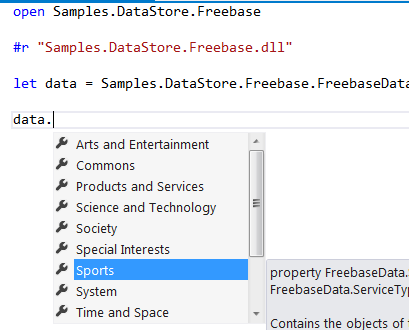
\includegraphics[width=0.95\linewidth]{tp-freebase.png}
  \Description{A screen shot of using the Freebase type provider. The autocomplete menu is shown for a data connection indicating the categories of information accessible.}
  \caption{Using the Freebase type provider.}
  \label{fig:freebase}
  \end{subfigure}
  \begin{subfigure}[b]{0.48\linewidth}
  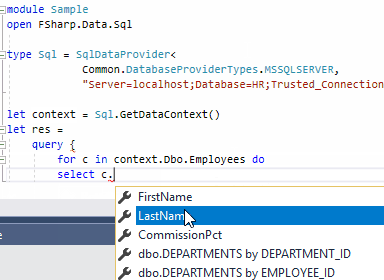
\includegraphics[width=0.95\linewidth]{sql-provider.png}
  \Description{A screen shot of using the SQL type provider. The autocomplete menu is shown for a data connection indicating the columns of information accessible.}
  \caption{Using a SQL type provider.}
  \label{fig:sql-provider}
  \end{subfigure}
  \caption{Two examples of integrating information sources into F\# using type providers, with strong typing and autocomplete.}


\end{figure}


This was F\# 2.0 but suddenly connected to immensely rich data sources, with IDE-integrated tooling.  Further, we were
doing these prototypes in the context of a language and tooling we could deliver “for real” to industry.  By June 2010 we
felt that we’d hit on somewhat of a goldmine for F\#. The feature addressed pragmatic customer concerns; was simple to
demonstrate; was innovative; avoided the need for bespoke tooling for different data sources; and allowed F\# to leap-frog
other languages in terms of data integration. Further, this feature could “transcend the divide” between research and product
and enable continued cooperation between MSR and the Microsoft product teams. 

In 2011 both MSR and Microsoft management committed to making type providers a major part of F\# 3.0. The period
between 2010 and 2012 was spent refining the mechanism and delivering a set of type-providers to work alongside F\#.
An online demonstrator called Try F\# was produced, funded by Tony Hey in Microsoft External Relations. F\# 3.0 also
included enhanced support for LINQ queries and a range of other improvements and fixes. Sarika Calla, Donna Malayeri
and Layla Driscoll took on program management responsibilities during this time and Donna acted as team lead.  Joe Palmer, Brian Macnamara, Dmitry
Lomov, Wonseok Chae and Vlad Matveev were development staff, and Matteo Taveggia, Tao Liu and
Jack Hu were QA staff (Figure~\ref{fig:team-2012-2014}). In 2011, Tao Liu presented the “F\# design patterns” on Channel 9.
Keith Battocchi (2011-13) and Ross McKinlay (2013) worked as contractors for Microsoft Research on applications of type
providers, developing applications of type providers potentially relevant to the Microsoft product line-up including integrating
Microsoft Dynamics CRM and Windows WMI computer management information and presenting at MSR TechFest 2012 and
2013.\footnote{Ross McKinlay is also famous in the F\# community for humorous applications of F\# type providers
including encoding “choose your own adventure” games in the autocomplete-menus made available to the programme
via the compile-time meta-programming machinery that integrates with the IDE \citep{RefChoose}.}

On release of F\# 3.0 on September 12, 2012,  F\# type providers immediately became a significant part of the F\# ecosystem, confirmed with the later creation of the FSharp.Data library of commonly-used type providers for XML, CSV and HTML data by Tomas Petricek and Gustavo Guerra.  Other applications of type providers include:

\begin{itemize}
\item Database integration (SQL)
\item Language integration (T-SQL, RProvider)
\item Configuration information integration (FSharp.Configuration)
\item Web APIs (via JSON and schematizations such as WSDL and Swagger)
\item Schematized “big-data” sources including Hadoop
\end{itemize}

The paper \textit{Types from data---Making structured data first-class citizens in F\#} \citep{Petricek2016} received a Distinguished Paper award at PLDI 2016 and was selected as one of three CACM Research Highlight in 2018.

\begin{figure}

  \centering
  \begin{subfigure}[b]{0.48\linewidth}
    
\includegraphics[width=\linewidth]{team-2012.jpg}
   \Description{Seven members of team shown outdoors}
  \end{subfigure}
  \begin{subfigure}[b]{0.48\linewidth}
    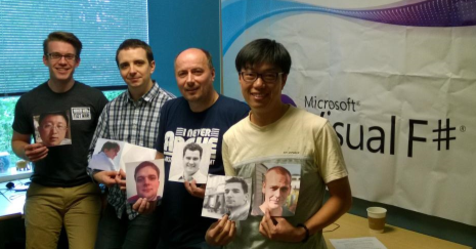
\includegraphics[width=\linewidth]{team-2014.png}
   \Description{Four members of team shown  indoors holding photos of others}
  \end{subfigure}
   \caption{Left: The F\# 3.0 Team, May 2012 (Don Syme, Jack Hu, Brian Macnamara, Vlad Matveev, Matteo Taveggia, Tao Liu, Wonseok Chae, Donna Malayeri).
Right: The F\# 4.0 Team, November 2014  (Lincoln Atkinson, Vlad Matveev, Kevin Ransom, Wonseok Chae), holding photos of 'community heroes' and open source contributors
including contributors Steffen Forkmann and Robert Jeppesen. (photos by Microsoft staff)}
  \label{fig:team-2012-2014}

\end{figure}




\section{.NET, F\# and the Shift to Cloud and Mobile Computing}

The focus of this paper is the early history of F\#, particularly up to F\# 3.0 in 2012 and the core set of innovative
features that have formed the backbone of all future versions of the F\# language. In the remainder of this paper, I
continue the more recent history since 2012, but in slightly less detail, particularly focusing on themes that were
present in the early history but where major changes have occurred.

Not all was plain sailing for F\#, C\# and .NET at Microsoft in the F\# 3.0 period.  This stemmed largely from seismic
shifts within the industry itself, with the rise of mobile and cloud computing.  The iPhone was launched in 2007 and a
massive change began in the industry. Around 2011, .NET hit serious hurdles inside Microsoft. For Windows 8, the
Windows team needed to reassess programmability in the light of the “consumer app” model being so successful on the
iPhone and iPad. As part of this, the Windows team decided to embrace HTML5 and JavaScript as a first-class language
for Windows programmability, and Windows 8 eventually supported C\#, JavaScript and C++ as the main programming
languages for “Windows Store” apps.  This was seen by many external observers as a “retreat” from .NET, even thoug
 C\# was the most popular language for Windows Store app development. This perception was reinforced when the
development of Silverlight, the browser-hosted version of .NET, was halted. Further, seeing the threat from the iPhone,
iPad and Android, the Windows team wanted to focus on consumer applications rather than enterprise.  

For F\# at Microsoft this posed a series of challenging issues. Within the company’s product range, F\# was positioned
as “functional programming for the enterprise” at a time where enterprise programming became less important to company
strategy, despite the enterprise sector sustaining up to 95\% of company profits through “platform pull-through”. For internal
political reasons, DevDiv didn’t feel able to push F\# as a choice for app programming on to the powerful Windows team.
Fortunately, F\# continued to receive good backing from DevDiv. While a reduction in resourcing occurred, and the pressure
was considerable, the team were given the resources to deliver the F\# 3.0 feature set at high quality, and
subsequently F\# 3.1 and so on.  Kevin Ransom joined the Visual F\# team along with team in February 2013, bringing depth of experience, having
worked on .NET and Visual Studio since its inception, and other team members were Wonseok Chae and Vlad Matveev (development), Layla Driscoll (PM),
Lincoln Atkinson (QA) and Gordon Hogenson (docs), and the team delivered F\# 3.1 plus multiple updates during 2013.
However, things were undoubtedly changing in the computing landscape and many
projects at Microsoft were affected. There was a causal connection from Apple's success with the iPhone resulting on pressure
on teams at Microsoft.  

Fortunately, around this time a major structural shift at Microsoft occurred with the development of the Azure cloud platform,
originally created in 2010 but achieving maturity and increasing commercial success from 2012.  A similar shift to commodity
computing on the server-side happened with platforms such as Amazon Web Services and Google Cloud Platform.   Cloud
programmability is highly suited to both high-level languages and functional programming, and from 2012 it became clear that
Azure and cloud computing was a critical part of the future of F\#. The same applied to .NET more generally, and Azure
became increasingly influential in the technical strategy for .NET, C\# and F\#.  Azure also drove a sea-change in Microsoft
as the company fully embraced open source for its programming languages, SDKs and tools used to access Azure. At this
time Microsoft also fully embraced the use of Linux within Azure---unthinkable a decade before.  Microsoft now “loved” Linux
and it formed a core part of one of its growth businesses.

During this time, the consultancy Nessos in Athens developed an innovative cloud programming system called MBrace
implemented in F\# \citep{Dzik2013}. Originally conceived as a distributed
programming system, later iterations emphasized cloud computing and big-data processing, and was used internally at
Microsoft to demonstrate the relevance of F\# for cloud programming. 


\section{A New Dawn for F\#, C\# and .NET: Open and Cross-Platform, At Last!}

F\# faced its most important and seemingly insurmountable challenge since its inception. Open-source software had
become the norm, and .NET, F\# and C\# were now definite outliers in the world of programming languages and
runtimes: largely closed source---or at least not accepting external contributions.  

At Microsoft there were many who advocated embracing open source, and the question had been lurking in the
background since the inception of .NET. In 2004 a “shared-source” version of .NET had been released. The source
for F\# had also been included with early MSR releases but on a non-commercial basis. However open source was
still controversial, and, in several instances, projects had been open-sourced only to be stopped soon
after.  “Going open” was thus still risky and needed to be explained carefully. 

On November 11, 2010, Microsoft made the first release of the F\# source under an OSI-approved
license (Apache 2.0), placing F\# in the vanguard of changes that would soon be embraced more widely \citep{RefCodeDrop}.
Even more importantly, on April 3, 2014 Microsoft started accepting contributions to F\#, which again “led the way” in embracing
a full open-engineering process \citep{RefOpenContrib}.
At Microsoft, Kevin Ransom and Lincoln Atkinson were key team members who made the transition to open source, open engineering and open design possible.
This also enabled a corresponding shift towards open-design and, with F\# 4.0, the
language shifted to an open and transparent design process \footnote{\textit{F\# Language Design RFCs}, \citep{RefRFCs}.}
The language design process and RFCs are now run through the FSSF under the guidance of myself, Phillip Carter (program manager for F\# at Microsoft) and Chet Husk.


The shift to openness had other effects too: in 2013 the .NET community finally developed a modern, effective way to
deliver packages through the creation of the NuGet package manager and the nuget.org package repository.  Prior to
this, the poor packaging story for .NET components was a major inhibitor to the growth of both .NET and F\#.  


Today, open-source is the norm for nearly all language and cloud tooling at Microsoft. The primary driving factor
behind this change is the increased focus on the Microsoft Azure cloud platform at Microsoft, with an economic basis in
selling services, rather than on selling packaged software and tools. C\#, .NET and F\# tooling accepts contributions and
has many contributors. Currently hosting over 120,000 packages, with nearly 10 billion package downloads, the NuGet
package ecosystem is rapidly growing to be one of the largest and most comprehensive in the world.  The open source ``Paket''
client has been a popular way to access this ecosystem for F\#
developers \citep{RefPaket}, and
the open source FAKE build scripting tool---where the build scripts are written in F\#---has been a “gateway drug” for the adoption of the language, allowing its
incremental adoption without rewriting the core of the project code \citep{RefFAKE}.

\section{The F\# Compiler as a Component}

In 2014 a technical breakthrough was made with the creation of the FSharp.Compiler.Service (FCS) package by
Tomas Petricek, Ryan Riley, and Dave Thomas with many later contributors \citep{RefFCS}.
This contains the core implementation of the F\# compiler, editor tooling and scripting engine in the form of a single library and can be used to make F\# tooling
for a wide range of situations.  This has allowed F\# to be delivered into many more editors, scripting and documentation
tools and allowed the development of alternative backends for F\#.   Key editor community-based tooling includes
Ionide, by Krzysztof Cieślak and contributors, used for rich editing support in the cross-platform VSCode editor, with over 1M downloads at time
of writing \citep{RefIonide}.

The FSharp.Compiler.Service component is a key enabler for consistent, performant cross-platform F\# language tooling in many different settings and
has few parallels amongst statically-typed  functional languages even today. It enables the F\# community to have the same set of language features working
similarly across different editors and on all platforms and also acts as a basis for tooling innovation in Ionide.

In 2018 the F\# community collaborated extensively with Microsoft on engineering processes, aligining code-repositories and
achieving efficient engineering practices.  Kevin Ransom, Phillip Carter, Brett Forsgren and Will Smith participated on the Microsoft side, and
many contributors from the broader F\# community.  The company Jet Brains also become extensive contributors to the F\# compiler and tools.
In 2019 Phillip Carter and Will Smith did extensive core performance work on the tooling to allow its use with very large F\# code bases.

\section{The F\# Community and the F\# Software Foundation }

\label{page:community}

The F\# community was initially sustained through hubFS.net forums (2005), created by Chris Barwick under the
pseudonym “optionsScalper”. The online Community for F\# (2007) was created by Ryan Riley which runs the
an F\# Heroes program \citep{RefCommunityFSharp}.
SkillsMatter London meetup in 2012 propelled the growth of the F\# community in the UK and Europe, and by 2018
over 50 F\# meetup groups have been created worldwide \citep{RefMeetupds}.
Community-run F\# conferences include openfsharp, F\# Exchange, F\# Europe and fableconf, and F\# material is regularly presented at both .NET-friendly and functional-friendly conferences. In 2011 the hubFS forums were replaced by FPish.net, implemented by Adam Granicz and others at IntelliFactory. 

\begin{wrapfigure}{R}{0.4\textwidth}
  \begin{center}
  
\includegraphics[width=0.8\linewidth]{fsharp-logo.png}
  \end{center}
  \caption{The F\# Logo of the F\# Software Foundation}
  \label{fig:fsharp-logo}
\end{wrapfigure}

In 2014, Tomas Petricek, Phil Trelford and myself met in a café in Cambridge and decided to start the F\# Software
Foundation (FSSF), commonly known as “fsharp.org”.  Initially this was an informal organization along the lines of the Python
Software Foundation.  An online meeting of potential community members was initiated, and Petricek and Trelford explained
their goals: a fun, open web-based organization that could represent the interests of F\# users.  Membership was free,
requiring only agreement with the mission statement of the organization, and grew quickly to about 500 members.  In 2016 the
FSSF incorporated as a U.S non-profit under the guidance of Reed Copsey and Mathias Brandewinder, and now holds yearly board elections. 

The formation of the FSSF was a highly significant moment for F\#.  Until then, a strong “culture of dependence” had existed in
large parts of the .NET and F\# communities, where users (including paying customers) expected Microsoft to solve all problems, provide all
resources and make all public communication about these technologies.  For example, many of those leading or participating
in F\# community activities were also Microsoft MVPs (Most Valued Professionals), and Microsoft ran either an F\#-specific or
.NET-specific MVP program from 2010 to the time of writing.  The F\# MVP program was both a major positive---for example, the
community was worldwide---but also a major negative, because it was not initially truly independent.
Parts of the F\# community had, however, successfully shifted to OSS and this led to the creation of the FSSF:
the F\# community now had a strong self-defining voice that could collect social proof, advocate for
the use of F\# and help guide community engineering efforts. As a result, F\# evangelism began to be more effective. One result of
the community’s more active role in evangelizing F\# was the creation of “F\# for Fun and Profit” by Scott Wlaschin, an impressive
collection of didactic material about functional programming concepts and practical F\# topics that has been very influential
in the F\# community \citep{RefFunAndProfit}.


The FSSF now has over 2000 members and owns fsharp.org and github.com/fsharp. The FSSF is now at the heart of the F\# community
and works with community stakeholders on F\# education, diversity, tooling, governance, mentorship, conference and software
initiatives.  The suggestions, RFCs and other documents related to the F\# language design process are hosted by the
FSSF \citep{RefRFCs, RefLangSuggestions}.

\section{.NET Core: Microsoft take C\#, F\# and .NET Cross-Platform}

The question of cross-platform support for .NET was present from the start: even the Rotor shared source release of 2004 was
cross-platform.  In 2001, the Mono project had been launched by Miguel de Icaza \cite{RefMono} and others to implement a fully open-source and
cross-platform version of .NET. F\# ran successfully on Mono since 2006.  

In 2016, Microsoft released a fully open-source and cross-platform implementation of .NET called .NET Core.  Since 2017, F\# support
is included directly in the .NET Core SDK and included in the standard Linux packages. With v2.0 released, .NET Core has been
increasingly successful, and the use of F\# on Linux and Docker is now mainstream within the community.  Cloud providers including
Amazon and Google now support F\# through .NET Core, which forms the backbone of .NET support in cloud-hosted services
such as Azure Functions, Amazon Lambda and Google Cloud Platform.

The inclusion of F\# directly in the .NET Core SDK is one the most significant long-term event in the history of the
language: F\# is now supported everywhere that the .NET Core SDK is installed, in a simple, consistent way and with full
backing from both an open source community and major commercial interests. Further, .NET Core has enabled the programming
framework to throw off some of the very tight constraints that came with backwards compatibility within the Windows
ecosystem, allowing rapid introduction of new features into the runtime layer. .NET Core allows side-by-side (i.e. non-interfering,
local) installations so installing updated runtimes does not affect existing applications on the same machine. This allows co-evolution
of the runtime and its languages (always one of the strong points of OCaml, which originally inspired F\#) and has already had
impact on the design of C\# and F\#, with the recent “Span” feature of C\# 7.2 and F\# 4.5 (allowing safe on-stack references
to interior sub-ranges of data such as strings) including both runtime and language elements.

\section{F\# for Mobile}


The industry shift to mobile and cloud computing saw a huge rise in the importance of Android and iOS as platforms from 2009
onwards.  With millions of people using .NET, a startup called Xamarin was formed to allow C\# and F\# developers to use their
existing skills to program apps for Android, iOS and Windows devices.  The Xamarin toolchain runs .NET IL code to interoperate
with Java (for Android) and Objective-C (for iOS).  Xamarin also provided cross-platform user interface programming options including Xamarin.Forms. 

Xamarin was eventually acquired by Microsoft and, as of 2018, F\# is a supported language in Microsoft’s mobile programming offerings.


\section{F\#, JavaScript and Full Stack Programming}

Since 2005 JavaScript has risen in importance as a delivery platform for programming languages. In 2007, Tomas Petricek
experimented with the first Javascript transpiler for F\#. In 2008 the first version of WebSharper was released, including
a more accurate and performant Javascript transpiler.  Innovative for its time, WebSharper is now a complete
open-source full-stack programming toolkit using F\# as its primary programming language.

In 2015 the F\# community also developed Fable, another JavaScript implementation of F\#, for web development
in the JS/Node ecosystem \citep{GarciaCaro2018}. At the time of writing, Fable is seeing increasing adoption for web
programming.  Fable became a key part of SAFE Stack, a “full stack” solution for F\# that incorporates web client, server and cloud
computing \citep{Abraham2020}.


\section{Retrospective}

In telling the genesis and early history of F\#, I positioned it as one of several “reactions” by those experienced
in strongly-typed functional programming to the tidal wave of Java and object-oriented programming that
engulfed the industry in the mid-1990s and the rise of the JVM and .NET.  In this light, F\# was in the vanguard
in changing how we deliver functional languages: F\# and Scala were among the first languages to be explicitly
designed and implemented on the assumption of an industry-standard runtime substrate such as the JVM or .NET.
With hindsight this decision was a good one and has subsequently been followed by many languages including
Clojure, Nemerle, Kotlin and Swift (the latter targeting the Objective-C runtime as substrate, with influence on the design of the language). A more recent
wave of languages has assumed JavaScript as a substrate, e.g. Elm, TypeScript and PureScript.  This approach is
now so common as to be industry-standard for new language efforts.

Programming languages get used for many purposes, and it would be impossible to do justice to the many fascinating
things people have done with F\#.  A key aspect of the early work of the FSSF was to collect and communicate
“social proof” about the effectiveness of F\# through testimonials \citep{FSharpTestimonials}.
Three uses are, however, particularly striking.
First, F\# was used to implement LIQUi|> (“Liquid”), a quantum simulator for F\#, by Dave Wecker and Microsoft
Quantum Computing.\citep{RefLiquid}. Second, F\# was used in conjunction with Rhinoceros3D to construct the digital 3D model
used in the manufacturing of the cladding of the Louvre Abu Dhabi Dome, a picture of which is included in Figure~\ref{fig:fig4}.
Thirdly, F\# was the primary language used at Jet.com, a start-up subsequently acquired by Walmart at a valuation
of over \$3B, and the first “unicorn” built using the Azure cloud platform. These alone constitute success for
strongly-typed functional programming of a scale undreamt of in 1998.

\begin{figure}

  
\includegraphics[width=0.8\linewidth]{fig4.jpg}
   \Description{A photo of an iconic architectural building with complex dome roof in the sunlight in Abu Dhabi}
  \caption{The Louvre Abu Dhabi---F\# was used for the digital 3D model to manufacture the roof (credit: Wikiemirati, Wikimedia, 29 April 2018, licensed under CC BY-SA 4.0, cropped)}
  \label{fig:fig4}

\end{figure}

Since around 2007 strongly-typed functional programming has shifted from relative obscurity to be a central paradigm
in programming. C\#, Java, C++, Scala, Kotlin, Swift, Rust and TypeScript now all include elements of
strongly-typed FP, and Apple executives extolled functional features at the launch of Swift in 2014, including
pattern matching, generics, option types, type inference, tuples and closures,
something unthinkable in 2005 \citep{RefSwift}. 
Haskell, F\# and OCaml have all grown in use, and newcomers such as Elm and ReasonML are also finding good adoption.

What caused this shift? Some factors have been touched on in this paper---for example, the relative decline of
widget-based GUI programming, and the corresponding rise of web programming, cloud computing, multi-core
programming and scalable-data processing, all of which are amenable to functional programming. The rise in importance
of JavaScript is also surely of relevance: although untyped it has many functional features. That said, it is noticeable
that the transition also seems to have started when Scala and F\# matured and received support at the heart of the
computing industry. More recent entrants such as Swift, ReasonML, TypeScript and Elm face many challenges,
but a lack of industry awareness of strongly-typed functional programming is not one of them. We’ve come a long
way since 1997, and Wadler’s question “Why no one uses functional programming?” has been consigned to the many short-lived curiosities of history.

\subsection{F\#'s Influence}

The most obvious direct influence of F\# has been on C\#. C\# 2.0 (generics) was based on preliminary work
by myself and others working on precursors to F\#, specifically with the intent of supporting ML-family
languages on .NET. C\# 3.0 (“var x = ...”), C\# 5.0 (tasks/async), C\# 7.0 (tuples, pattern matching),
C\# 8.0 (enhanced pattern matching) and C\# 9.0 (non-null pointers as the default) were all heavily influenced by F\# \citep{RefUseFSharp}. Given that C\# is one of
the most widely adopted languages today, and underwent rapid iteration in the 2000s\footnote{The language designs of Java, C++, JavaScript and Python
all progressed during this time, but to a lesser extent than C\#.}, it is reasonable to
claim that the presence of F\# within the Microsoft Developer Division played an important role as a bridge
between the stream of ideas that constitute “functional programming” and C\#.   That said, the ideas have
flowed both ways, with F\# also influenced by C\# 1.0 (objects, properties, events), C\# 3.0 (LINQ) and C\# 7.0 (Span).
There have also been influences on C\# from other sources such as Icon (C\# 2.0 Iterators), Python (C\# 4.0 Dynamic) and
the internal projects Axum by Gustafsson et al. \citep{RefAxum}.

The addition of first-class events and compositional event-combinator programming to F\# influenced directly the initiation
of the Rx project, a reactive-functional programming toolkit now re-implemented as a pattern in multiple languages
including Rx.JS \citep{RefFirstClassEventsBlog}.  The early influence of F\# here was recounted informally to me by Wes Dyer. 

Other direct influences of F\# on languages are harder to measure: language designers tend to be coy about their
influences both direct and indirect. Both Elixir and Elm use the \texttt{|>} operator and there are ways to emulate that operator
in other languages such as Scala and R. The Scala designer, Martin Odersky, was intimately aware of F\# throughout
its history in his role on the MSR Cambridge Technical Advisory Board and EPFL research includes efforts to
bring F\# type providers to Scala \citep{Burmako2013}.  The apparent influence of F\# on the
creation of Scala extractors was mentioned earlier in this article and Scala 3.0 later adopted indentation-aware 
syntax. Swift seems to have been influenced
by F\#, and Joe Pamer managed the team at Apple responsible for developing the Swift compiler from 2014-16.
Kotlin seems to use C\#, F\# and other languages as reference points.  Rust seems to have been
influenced by OCaml, and the author Graydon Hoare refers to F\# extensively when discussing “What’s Next” after
Rust \citep{RefGraydon}.
TypeScript was directly influenced by F\#: one of the originators of TypeScript was
Luke Hoban, who began TypeScript (then called Strada) immediately after working on F\# 2.0. Recently
he noted the influence of F\# on early parts of the TypeScript
design \citep{RefTypeScriptDemo}. The
extent and nature of this influence is a matter of debate, but it is my opinion that TypeScript is firmly based on positive experience of advanced type checking and inference
in the context of F\#, and would not have appeared from a Microsoft team in anything close to its current form without the influence of F\#.

From the outset, F\# placed non-nullness as central to its design: the value “null” can’t normally be used in conjunction
with F\#-declared types, and in practice null-reference exceptions are rare.\footnote{The F\# community joke being “Question: What can C\# do that F\# can’t?” “Answer: NullReferenceException!”}   This affects many micro-decisions in the
language. Coming from the OCaml perspective, this is an obvious choice, and in the cultural context of MSR
Cambridge---including the presence of Tony Hoare at the lab and the memory of his “Billion Dollar Mistake”---any
other choice would have been unthinkable \citep{HoareNulls2011}.  However, languages like Scala didn’t make the same
decision, and even by 2018 F\# was the only significant language running on the JVM or .NET that placed non-nullness
as central to its design. At the time of writing, in February 2020, C\# 9.0 is planning to make non-nullness the
default, a dramatic shift that I hope will herald a shift to eliminate this endemic problem from the programming industry. F\# has been central to this process.

F\# was the first language to introduce an “async” modality to allow the localized reinterpretation of the existing
control constructs of the language. This meant that converting a piece of code from “synchronous” to
“asynchronous” involved nothing more than wrapping \texttt{async \{ ... \}} around the code and marking up
the “await” points (\texttt{let!} in F\#).   This directly influenced the async/await mechanism added to C\# 5.0 in 2012---the
F\# version was first presented to the C\# designers in 2007 and many discussions were held in
between.  The C\# async/await feature has been influential on TypeScript, Kotlin, Python 3.5, Java, JavaScript and other
languages.\footnote{The history of async programming, continuations and co-routines would need to be the subject
of a different article, stretching back to LISP. The influence of MLDonkey
on F\# has been noted earlier. C\# 5.0 added new elements to the design
of “async/await” suitable for an ALGOL language, including state-machine compilation,
derived originally from the Axum prototype noted earlier.  In this light, F\# async was a
precursor to C\# async/await, and the latter was not a simple copy of the former.}
Having an async modality in a language is now effectively an industry standard, and in each case the lineage of this
feature traces back partly through F\#.

In short F\# has influenced many of the major languages in use as of 2020, either directly (C\#, TypeScript, Scala, Kotlin, possibly Swift) or
indirectly (Rust, Python, Java, JavaScript), with the possible exception of C++.

\subsection{Mistakes and Questions}

Mistakes are hard to admit, and best seen in their historical context.  From the early history,
the greatest mistake related to F\# was that neither .NET nor the language were open source
or using open engineering.  This mistake was well-understood by the core contributors at the time
and many across Microsoft were advocating for a shift to open-source. Put simply, an innovative language
grew in the research lab of a company that had not yet embraced open source: those involved did
what they could through source drops, and the problem was eventually solved via the shift to open
source engineering and design from 2011 to 2014. The rectification of this mistake will likely be
the most significant development in the history of the language. Further, the fact
that F\# was able to navigate 2002-2011 while using closed-engineering is largely due to the
recognition of its qualities by decision makers at Microsoft.

One unfortunate side effect of closed-engineering was discontinuity: most early
contributors to F\# soon moved on to other jobs. Because F\# was not open source, they
were unable to continue to contribute to the codebase, even transitionally. Today, contributors
can come and go freely and frequently answer questions about older code.

From a technical perspective, F\# has made many contributions, yet the core feature set has
been stable and even binary-compatible since F\# 1.9.  There are, of course, some
design mistakes, including active bugs.  Of these, the “statically resolved type parameter”
mechanism is perhaps the one causing most corner-case niggles. Originally designed just for
operator overloading, the mechanism is also used by some advanced F\# users as a type constraint
mechanism akin to Haskell type classes. Perhaps more concerningly, it is also used extensively
and inappropriately by some beginner F\# users or those in teams, attempting to
over-apply "maximal abstraction" DRY (Don't Repeat Yourself) techniques in coding.   The combination of complex SRTP constraints
with algorithm-based type inference is, however, fragile, and it is proving hard to fix some
mistakes in the resolution of SRTP constraints without breaking some existing code in
corner cases.  If backwards compatibility were not a major concern this would not be
a problem, however it is highly valued by both the F\# community and Microsoft design groups.

The design of F\# incorporated some features of OCaml which, in retrospect, could have
been omitted.  One example is generic comparison: OCaml supports unconstrained generic
structural operators \texttt{=}, \texttt{<>}, \texttt{<}, \texttt{>}, \texttt{<=}, \texttt{>=}, \texttt{compare}, \texttt{min} and \texttt{max}.
The F\# design enforces “equality” and “comparable” type constraints on these operators, but the runtime
implementation of generic comparison is complicated, particularly because of corner cases
such as NaN on floating point numbers. There are also performance implications when
using these operators. In retrospect, the whole generic comparison feature could likely
have been omitted from F\#, or greatly constrained.

One recurring theme of F\# language evolution has been its interaction with corresponding
C\# and .NET design elements.  For example, F\# 1.9 added Async<T> in 2007.  In
contrast, .NET added \texttt{Task<T>} in 2010 and C\# 5.0 added language integrated support for \texttt{Task<T>} in
2012.  At the high level these are all “the same thing”, i.e. lightweight user-level threading. However,
even at the time of writing, in 2019, these sit awkwardly together. They interoperate:
you can generate \texttt{Task<T>} from an \texttt{Async<T>}, and await a \texttt{Task<T>} in an \texttt{Async<T>}, but
each has distinct advantages. For example, when using \texttt{Async<T>}, the F\# programmer is relieved of the burden of
passing cancellation tokens explicitly, and, when using \texttt{Task<T>}, performance is better with fewer allocations.  

This tension, where F\# added one version of a feature, only for C\# to add a modified version of a similar
feature later, was repeated even with tuples: F\# had boxed tuples from the outset in 2002,
and C\# added unboxed tuples in 2017.  In 2017 the F\# design team had to
adjust F\# to allow both boxed and unboxed tuples. The introduction of C\# expression quotations in
2007 was similar: F\# had quotations Expr<T>, but C\#’s expression quotation added
LINQ’s \texttt{Expression<T>}, widely used by .NET libraries. C\# expressions quotations are strictly
more limited than F\# quotations (covering only C\# expressions, and not statement forms), and
more complicated, but they are effectively a .NET standard.  To my knowledge no other language
dances quite so closely with a “bigger” language. It is important for the long-term integrity of the F\# design
that these adjustments are done with extreme care.

One small but fortuitous mistake was the precedence of the “back-piping”
operator \verb$f <| x$, which can’t be used in iterated fashion \verb$f2 <| f1 <| x$ due to
a left-associative precedence. This was not deliberate---the precedence was simply
taken from OCaml---but was never fixed because the preferred F\# style is  \verb$x |> f1 |> f2$. The
mistake has the benefit of restricting the use of the operator which rarely results in readable code. The F\# library also includes
multi-argument back-piping operators \verb$<||$ and \verb$<|||$ which should never have been included simply for
stylistic reasons: code using them is very rare but also incomprehensible.

As a language design, F\# has many opportunities to evolve, and over 200 active language
suggestions are recorded on the “F\# Language Suggestions” site that forms part of the
official FSSF language design process \citep{RefLangSuggestions}.
Two of the most popular suggestions are type classes
and higher kind type parameterization. However, in both cases I’ve indicated an unwillingness
to add this feature to F\# without also adding a matching feature to C\#, partly to avoid a
recurring pattern of multiple semi-compatible versions of similar features.

As indicated in the discussion on .NET Core, significant evolution steps are likely to happen in
conjunction with the design of both C\# and the .NET runtime itself.  One example is the addition
of safe high-performance memory primitives called “Span” in F\# 4.5 and C\# 7.2.  This feature
had the added benefit of helping iron out various minor problems present since the F\# 2.0 design.

\section{Conclusion}

In this article, I have tried to sketch the long arc from Robin Milner in the 1970s to F\# as it
is today, with a focus on the genesis and early history of F\# and the context in which
that happened. F\# has come a long way since 2001, when it was an idea in
an email on the OCaml mailing list, or 2006, when it was a Microsoft Research project,
or 2010, when F\# 2.0 was effectively tied to Windows. The core spirit of ML---succinct,
type-safe, correct, pragmatic, functional-first programming---has held true throughout
this journey, with the integration of new ideas along the way.  F\# today is open-source
and cross-platform, with both commercial support and a vibrant community. It has a solid future
evolution path and is usable as a practical and enjoyable functional-first programming language in many application domains.  





%% Acknowledgments
\begin{acks}                            %% acks environment is optional
                                        %% contents suppressed with 'anonymous'

Many thanks to Andrea Magnorsky, Phillip Carter, Phillip Haller, Darren Platt, Natallie Baikevich, Richard Campbell, Adam Granicz, Tomas Petricek, Miguel de Icaza, Phillip Wadler, Mark Staples, Robert Pickering, Simon Peyton Jones, Krzysztof Cieślak, Stafford Williams, Dov Murik, Ryan Riley   and many others for feedback on early drafts of this paper.  Mark Laws helped prepare the camera-ready copy, for which I am very grateful. Any mistakes that remain are my responsibility. Please contact me with extra information or corrections.

  %% Commands \grantsponsor{<sponsorID>}{<name>}{<url>} and
  %% \grantnum[<url>]{<sponsorID>}{<number>} should be used to
  %% acknowledge financial support and will be used by metadata
  %% extraction tools.
%  This material is based upon work supported by the
  %\grantsponsor{GS100000001}{National Science
    %Foundation}{http://dx.doi.org/10.13039/100000001} under Grant
  %No.~\grantnum{GS100000001}{nnnnnnn} and Grant
 % No.~\grantnum{GS100000001}{mmmmmmm}.  Any opinions, findings, and
  %conclusions or recommendations expressed in this material are those
 % of the author and do not necessarily reflect the views of the
  %National Science Foundation.
\end{acks}


%% Bibliography
\bibliography{bib}


%% Appendix
%\appendix
%\section{Appendix}
%
%Text of appendix \ldots

\end{document}
